\documentclass[]{article}
\usepackage{lmodern}
\usepackage{amssymb,amsmath}
\usepackage{ifxetex,ifluatex}
\usepackage{fixltx2e} % provides \textsubscript
\ifnum 0\ifxetex 1\fi\ifluatex 1\fi=0 % if pdftex
  \usepackage[T1]{fontenc}
  \usepackage[utf8]{inputenc}
\else % if luatex or xelatex
  \ifxetex
    \usepackage{mathspec}
  \else
    \usepackage{fontspec}
  \fi
  \defaultfontfeatures{Ligatures=TeX,Scale=MatchLowercase}
\fi
% use upquote if available, for straight quotes in verbatim environments
\IfFileExists{upquote.sty}{\usepackage{upquote}}{}
% use microtype if available
\IfFileExists{microtype.sty}{%
\usepackage{microtype}
\UseMicrotypeSet[protrusion]{basicmath} % disable protrusion for tt fonts
}{}
\usepackage[margin=1in]{geometry}
\usepackage{hyperref}
\hypersetup{unicode=true,
            pdftitle={BMIN503 Final Project: Disparities in managing migraine pain in the pediatric ER},
            pdfauthor={Sansanee Craig},
            pdfborder={0 0 0},
            breaklinks=true}
\urlstyle{same}  % don't use monospace font for urls
\usepackage{color}
\usepackage{fancyvrb}
\newcommand{\VerbBar}{|}
\newcommand{\VERB}{\Verb[commandchars=\\\{\}]}
\DefineVerbatimEnvironment{Highlighting}{Verbatim}{commandchars=\\\{\}}
% Add ',fontsize=\small' for more characters per line
\usepackage{framed}
\definecolor{shadecolor}{RGB}{248,248,248}
\newenvironment{Shaded}{\begin{snugshade}}{\end{snugshade}}
\newcommand{\KeywordTok}[1]{\textcolor[rgb]{0.13,0.29,0.53}{\textbf{#1}}}
\newcommand{\DataTypeTok}[1]{\textcolor[rgb]{0.13,0.29,0.53}{#1}}
\newcommand{\DecValTok}[1]{\textcolor[rgb]{0.00,0.00,0.81}{#1}}
\newcommand{\BaseNTok}[1]{\textcolor[rgb]{0.00,0.00,0.81}{#1}}
\newcommand{\FloatTok}[1]{\textcolor[rgb]{0.00,0.00,0.81}{#1}}
\newcommand{\ConstantTok}[1]{\textcolor[rgb]{0.00,0.00,0.00}{#1}}
\newcommand{\CharTok}[1]{\textcolor[rgb]{0.31,0.60,0.02}{#1}}
\newcommand{\SpecialCharTok}[1]{\textcolor[rgb]{0.00,0.00,0.00}{#1}}
\newcommand{\StringTok}[1]{\textcolor[rgb]{0.31,0.60,0.02}{#1}}
\newcommand{\VerbatimStringTok}[1]{\textcolor[rgb]{0.31,0.60,0.02}{#1}}
\newcommand{\SpecialStringTok}[1]{\textcolor[rgb]{0.31,0.60,0.02}{#1}}
\newcommand{\ImportTok}[1]{#1}
\newcommand{\CommentTok}[1]{\textcolor[rgb]{0.56,0.35,0.01}{\textit{#1}}}
\newcommand{\DocumentationTok}[1]{\textcolor[rgb]{0.56,0.35,0.01}{\textbf{\textit{#1}}}}
\newcommand{\AnnotationTok}[1]{\textcolor[rgb]{0.56,0.35,0.01}{\textbf{\textit{#1}}}}
\newcommand{\CommentVarTok}[1]{\textcolor[rgb]{0.56,0.35,0.01}{\textbf{\textit{#1}}}}
\newcommand{\OtherTok}[1]{\textcolor[rgb]{0.56,0.35,0.01}{#1}}
\newcommand{\FunctionTok}[1]{\textcolor[rgb]{0.00,0.00,0.00}{#1}}
\newcommand{\VariableTok}[1]{\textcolor[rgb]{0.00,0.00,0.00}{#1}}
\newcommand{\ControlFlowTok}[1]{\textcolor[rgb]{0.13,0.29,0.53}{\textbf{#1}}}
\newcommand{\OperatorTok}[1]{\textcolor[rgb]{0.81,0.36,0.00}{\textbf{#1}}}
\newcommand{\BuiltInTok}[1]{#1}
\newcommand{\ExtensionTok}[1]{#1}
\newcommand{\PreprocessorTok}[1]{\textcolor[rgb]{0.56,0.35,0.01}{\textit{#1}}}
\newcommand{\AttributeTok}[1]{\textcolor[rgb]{0.77,0.63,0.00}{#1}}
\newcommand{\RegionMarkerTok}[1]{#1}
\newcommand{\InformationTok}[1]{\textcolor[rgb]{0.56,0.35,0.01}{\textbf{\textit{#1}}}}
\newcommand{\WarningTok}[1]{\textcolor[rgb]{0.56,0.35,0.01}{\textbf{\textit{#1}}}}
\newcommand{\AlertTok}[1]{\textcolor[rgb]{0.94,0.16,0.16}{#1}}
\newcommand{\ErrorTok}[1]{\textcolor[rgb]{0.64,0.00,0.00}{\textbf{#1}}}
\newcommand{\NormalTok}[1]{#1}
\usepackage{graphicx,grffile}
\makeatletter
\def\maxwidth{\ifdim\Gin@nat@width>\linewidth\linewidth\else\Gin@nat@width\fi}
\def\maxheight{\ifdim\Gin@nat@height>\textheight\textheight\else\Gin@nat@height\fi}
\makeatother
% Scale images if necessary, so that they will not overflow the page
% margins by default, and it is still possible to overwrite the defaults
% using explicit options in \includegraphics[width, height, ...]{}
\setkeys{Gin}{width=\maxwidth,height=\maxheight,keepaspectratio}
\IfFileExists{parskip.sty}{%
\usepackage{parskip}
}{% else
\setlength{\parindent}{0pt}
\setlength{\parskip}{6pt plus 2pt minus 1pt}
}
\setlength{\emergencystretch}{3em}  % prevent overfull lines
\providecommand{\tightlist}{%
  \setlength{\itemsep}{0pt}\setlength{\parskip}{0pt}}
\setcounter{secnumdepth}{0}
% Redefines (sub)paragraphs to behave more like sections
\ifx\paragraph\undefined\else
\let\oldparagraph\paragraph
\renewcommand{\paragraph}[1]{\oldparagraph{#1}\mbox{}}
\fi
\ifx\subparagraph\undefined\else
\let\oldsubparagraph\subparagraph
\renewcommand{\subparagraph}[1]{\oldsubparagraph{#1}\mbox{}}
\fi

%%% Use protect on footnotes to avoid problems with footnotes in titles
\let\rmarkdownfootnote\footnote%
\def\footnote{\protect\rmarkdownfootnote}

%%% Change title format to be more compact
\usepackage{titling}

% Create subtitle command for use in maketitle
\newcommand{\subtitle}[1]{
  \posttitle{
    \begin{center}\large#1\end{center}
    }
}

\setlength{\droptitle}{-2em}

  \title{BMIN503 Final Project: Disparities in managing migraine pain in the
pediatric ER}
    \pretitle{\vspace{\droptitle}\centering\huge}
  \posttitle{\par}
    \author{Sansanee Craig}
    \preauthor{\centering\large\emph}
  \postauthor{\par}
      \predate{\centering\large\emph}
  \postdate{\par}
    \date{December 11, 2018}


\begin{document}
\maketitle

\subsection{Overview}\label{overview}

Racial disparities in pain management have been documented in the adult
and pediatric population. Most studies have focused on pathologies with
definitive diagnostic testing, such as appendicitis, long-bone
fractures, and sickle cell disease. Few studies have assessed
variability of pain management in pediatric migraine. The purpose of
this project is to utilize secondary analysis of EHR data to determine
if race/ethnicity-based differences exist in the management of pediatric
migraine pain in the emergency room at the Children’s Hospital of
Philadelphia (CHOP).

\subsection{Introduction}\label{introduction}

Pain management cross-sects most fields of medical practice. In the case
of migraine pain, a patient’s care team may comprise a primary care
physician and a neurologist, with ER and hospitalist providers added
during refractory migraine episodes. Alleviating pain efficiently,
safely, and equally for all patients is the ultimate goal during an
emergency room visit. In the few pediatric studies to date, however,
some sociodemographic disparities have been shown to exist in pediatric
headache care across the United States.\\
In beginning to study this issue, thoughtful data queries in conjunction
with data analysts is vital as the choices behind codifying race and
ethnicity alone could significantly alter study results. Workflow
analysis during direct observations in the ER provides insight into
missing field factors, such as non-mandatory data entry in assigning a
pain scale/score or completing demographic fields. Nurses’ feedback
sheds light on why pain reassessment alerts were being ignored or pain
scales not being assigned during registration. Discussions with ER
physicians and the ER director provides background information on
previous disparities study results and QI projects, identifying most
relevant outcome to study, and factors in choosing which statistical
result to report. Meeting with a pediatric neurologist, the director of
the headache clinic, results in an additional view of focusing QI
efforts on giving primary care providers better tools to care for
migraine pain in order to decrease unnecessary neurology referrals or ER
visits. In short, data scientists and quality improvement (QI) teams can
contribute to understanding the best methods to study where these
disparities lie and how to rapidly conduct improvement projects to
decrease known disparities. Clinical informaticists help to facilitate
change management by navigating the socio-technical factors in hospital
and clinic organizations. Thus, this is a multidisciplinary project with
stakeholders spanning the field biomedical and health informatics.

\subsection{Methods}\label{methods}

The data used in this project were imported as a CSV file from Qlikview,
a software that displays results from SQL queries written by CHOP data
analysts. This SQL query specifically pulls data from the CHOP EMR
(Epic) on patients ages 5 -18 who were treated with the migraine pain
order set in the CHOP ER. Results exported as .xlsx file were
de-identified before saving as a .csv file for import to R. All data
available in Qlikview were imported without filtering. One observation
was noted to be missing MRN and 20 other variables, so was assumed error
and deleted before import.

\subsubsection{Data loading and
cleaning}\label{data-loading-and-cleaning}

\paragraph{Load data set, assign NA's, transform variable
classes}\label{load-data-set-assign-nas-transform-variable-classes}

\begin{Shaded}
\begin{Highlighting}[]
\NormalTok{data_all<-}\StringTok{ }\KeywordTok{read.csv}\NormalTok{(}\StringTok{"https://raw.githubusercontent.com/scraig10/BMIN503_Final_Project/master/data_all_11_28_2018.csv"}\NormalTok{, }\DataTypeTok{header=}\OtherTok{TRUE}\NormalTok{)}
\KeywordTok{str}\NormalTok{(data_all) }\CommentTok{# 3709 observations of 33 variables}
\end{Highlighting}
\end{Shaded}

\begin{verbatim}
## 'data.frame':    3709 obs. of  33 variables:
##  $ X                                : int  1 2 3 4 5 6 7 8 9 10 ...
##  $ ED.Arrive                        : Factor w/ 3709 levels "1/1/2016 12:23",..: 998 997 993 992 985 984 983 968 967 966 ...
##  $ ED.LOS..min.                     : Factor w/ 638 levels "-","1,018","1,022",..: 163 1 195 193 477 49 178 121 88 141 ...
##  $ Pathway                          : Factor w/ 2 levels "No","Yes": 2 2 2 2 2 2 2 2 2 2 ...
##  $ Sex                              : Factor w/ 2 levels "F","M": 2 1 1 2 1 1 1 1 1 2 ...
##  $ Race.Ethnicity                   : Factor w/ 4 levels "HISPANIC OR LATINO",..: 4 1 3 2 2 4 1 3 2 3 ...
##  $ Payer.Type                       : Factor w/ 3 levels "-","COMMERCIAL",..: 2 3 3 3 3 2 2 2 3 2 ...
##  $ Primary.Language                 : Factor w/ 2 levels "ENGLISH","NON-ENGLISH": 1 1 1 1 1 1 1 1 1 1 ...
##  $ Acuity                           : Factor w/ 5 levels "1 Critical","2 Acute",..: 3 3 3 3 3 4 3 3 3 3 ...
##  $ CCC                              : Factor w/ 2 levels "No","Yes": 1 1 2 2 2 2 1 2 1 2 ...
##  $ HCG                              : Factor w/ 2 levels "No","Yes": 1 1 2 1 2 1 2 2 2 1 ...
##  $ HCG.Result                       : Factor w/ 1830 levels "-","1/1/2015 0:31",..: 1 1 493 1 1 1 492 484 483 1 ...
##  $ Arrive.to.Room                   : int  11 32 12 3 2 4 3 5 10 4 ...
##  $ Room.to.MD.Eval                  : int  30 31 12 23 1 10 7 3 2 4 ...
##  $ MD.Eval.to.First.Med.Order       : Factor w/ 299 levels "-","-1","-10",..: 176 1 1 244 227 185 222 181 162 211 ...
##  $ X1st.Med.Ordered.to.Started      : Factor w/ 164 levels "-","-1","-1,170",..: 99 1 1 64 38 79 95 115 107 64 ...
##  $ X1st.Med.Started.to.Given        : Factor w/ 259 levels "-","0","1","1,000",..: 127 1 1 68 250 2 259 96 115 2 ...
##  $ Bolus.Start                      : Factor w/ 2861 levels "-","1/1/2015 2:31",..: 762 1 1 760 759 1 753 741 740 1 ...
##  $ Toradol.Given                    : Factor w/ 2555 levels "-","1/1/2015 2:41",..: 1 1 1 686 687 1 681 1 670 1 ...
##  $ Reglan.Start                     : Factor w/ 2930 levels "-","1/1/2015 2:42",..: 781 1 1 777 778 770 1 755 754 753 ...
##  $ Reglan.Given                     : Factor w/ 2933 levels "-","1/1/2015 2:42",..: 779 1 1 775 776 768 1 753 752 751 ...
##  $ Reglan.Infusion.Time             : Factor w/ 130 levels "-","-17","-7",..: 27 1 1 124 62 4 1 27 27 4 ...
##  $ Reglan.Route                     : Factor w/ 4 levels "-","Intravenous",..: 2 1 1 2 2 4 1 2 2 4 ...
##  $ Arrive.to.1st.Med.Given          : Factor w/ 398 levels "-","100","101",..: 26 1 1 352 318 345 77 2 395 335 ...
##  $ X1st.Med.Reassessment            : Factor w/ 219 levels "-","100","101",..: 182 1 1 206 182 1 1 14 1 1 ...
##  $ X1st.Med.Given.to.2nd.Med.Ordered: Factor w/ 319 levels "-","-1","-10",..: 1 1 1 1 1 1 1 1 1 1 ...
##  $ Initial.2nd.Med.Given            : Factor w/ 4 levels "-","MAGNESIUM SULFATE",..: 1 1 4 1 1 1 1 1 1 1 ...
##  $ X2nd.Med.Reassessment            : Factor w/ 180 levels "-","100","101",..: 1 1 97 1 1 1 1 1 1 1 ...
##  $ X2nd.Meds.Given                  : Factor w/ 9 levels "-","ALL","MAGNESIUM SULFATE",..: 6 1 7 6 6 6 6 6 6 6 ...
##  $ X72hr.Revisit                    : Factor w/ 2 levels "No","Yes": 1 1 1 1 1 1 1 1 1 1 ...
##  $ X7d.Revisit                      : Factor w/ 2 levels "No","Yes": 1 1 1 1 1 1 1 1 1 1 ...
##  $ Dispo                            : Factor w/ 2 levels "Admitted","Discharged": 2 2 1 2 2 2 2 2 2 2 ...
##  $ Team.Assessment.                 : Factor w/ 3 levels "-","0","1": 2 2 2 2 2 2 2 2 2 2 ...
\end{verbatim}

\begin{Shaded}
\begin{Highlighting}[]
\KeywordTok{summary}\NormalTok{(data_all) }\CommentTok{#First glance, it seems there are no missing variables. }
\end{Highlighting}
\end{Shaded}

\begin{verbatim}
##        X                  ED.Arrive     ED.LOS..min.  Pathway    Sex     
##  Min.   :   1   1/1/2016 12:23 :   1   213    :  22   No : 645   F:2615  
##  1st Qu.: 928   1/1/2017 11:18 :   1   255    :  22   Yes:3064   M:1094  
##  Median :1855   1/10/2014 12:17:   1   199    :  20                      
##  Mean   :1855   1/10/2016 18:34:   1   261    :  20                      
##  3rd Qu.:2782   1/10/2016 19:26:   1   216    :  19                      
##  Max.   :3709   1/10/2017 14:10:   1   204    :  18                      
##                 (Other)        :3703   (Other):3588                      
##             Race.Ethnicity              Payer.Type      Primary.Language
##  HISPANIC OR LATINO: 264   -                 : 112   ENGLISH    :3641   
##  NON-HISPANIC BLACK:1514   COMMERCIAL        :2089   NON-ENGLISH:  68   
##  NON-HISPANIC WHITE:1750   MEDICAL ASSISTANCE:1508                      
##  OTHER             : 181                                                
##                                                                         
##                                                                         
##                                                                         
##           Acuity      CCC        HCG                  HCG.Result  
##  1 Critical  :   7   No :2095   No :1664   -               :1873  
##  2 Acute     : 623   Yes:1614   Yes:2045   1/31/2015 19:01 :   2  
##  3 Urgent    :2753                         11/7/2014 11:55 :   2  
##  4 Urgent    : 312                         12/11/2017 21:18:   2  
##  5 Non-Urgent:  14                         2/25/2014 20:26 :   2  
##                                            3/24/2015 10:20 :   2  
##                                            (Other)         :1826  
##  Arrive.to.Room   Room.to.MD.Eval  MD.Eval.to.First.Med.Order
##  Min.   :-56.00   Min.   :-15.00   -      : 451              
##  1st Qu.:  4.00   1st Qu.:  3.00   19     :  67              
##  Median :  9.00   Median :  9.00   20     :  63              
##  Mean   : 24.84   Mean   : 19.41   23     :  61              
##  3rd Qu.: 29.00   3rd Qu.: 26.00   29     :  59              
##  Max.   :405.00   Max.   :293.00   26     :  58              
##                                    (Other):2950              
##  X1st.Med.Ordered.to.Started X1st.Med.Started.to.Given
##  -      : 451                0      : 563             
##  21     :  90                -      : 451             
##  27     :  89                1      :  75             
##  26     :  88                20     :  71             
##  24     :  87                21     :  63             
##  23     :  83                18     :  61             
##  (Other):2821                (Other):2425             
##           Bolus.Start            Toradol.Given            Reglan.Start 
##  -              : 846   -               :1153   -               : 771  
##  1/30/2015 9:00 :   2   12/17/2014 21:14:   2   1/28/2014 15:30 :   2  
##  3/17/2014 21:30:   2   3/7/2016 15:45  :   2   10/9/2017 12:16 :   2  
##  9/7/2017 13:30 :   2   1/1/2015 2:41   :   1   11/11/2014 17:39:   2  
##  1/1/2015 2:31  :   1   1/1/2016 13:38  :   1   12/10/2015 18:19:   2  
##  1/1/2016 13:43 :   1   1/1/2017 17:44  :   1   12/16/2015 14:45:   2  
##  (Other)        :2855   (Other)         :2549   (Other)         :2928  
##            Reglan.Given  Reglan.Infusion.Time         Reglan.Route 
##  -               : 771   0      :1297         -             : 771  
##  1/28/2014 15:30 :   2   -      : 771         Intravenous   :2505  
##  1/28/2016 16:44 :   2   15     : 325         NOT APPLICABLE:   1  
##  10/9/2017 12:16 :   2   20     :  89         Oral          : 432  
##  11/11/2014 17:39:   2   16     :  60                              
##  12/16/2015 15:00:   2   30     :  57                              
##  (Other)         :2928   (Other):1110                              
##  Arrive.to.1st.Med.Given X1st.Med.Reassessment
##  -      : 451            -      :1278         
##  153    :  31            44     :  54         
##  102    :  29            46     :  46         
##  131    :  29            42     :  44         
##  109    :  28            36     :  41         
##  113    :  28            37     :  40         
##  (Other):3113            (Other):2206         
##  X1st.Med.Given.to.2nd.Med.Ordered        Initial.2nd.Med.Given
##  -      :2607                      -                 :2600     
##  49     :  20                      MAGNESIUM SULFATE :  70     
##  37     :  16                      METHYLPREDNISOLONE: 292     
##  72     :  16                      VALPROATE         : 747     
##  53     :  14                                                  
##  50     :  13                                                  
##  (Other):1023                                                  
##  X2nd.Med.Reassessment                      X2nd.Meds.Given X72hr.Revisit
##  -      :2973          NONE                         :2406   No :3600     
##  20     :  18          VALPROATE                    : 463   Yes: 109     
##  60     :  16          VALPROATE, METHYLPREDNISOLONE: 273                
##  31     :  15          -                            : 194                
##  32     :  14          METHYLPREDNISOLONE           : 172                
##  55     :  14          ALL                          :  75                
##  (Other): 659          (Other)                      : 126                
##  X7d.Revisit        Dispo      Team.Assessment.
##  No :3524    Admitted  : 597   -:   4          
##  Yes: 185    Discharged:3112   0:3414          
##                                1: 291          
##                                                
##                                                
##                                                
## 
\end{verbatim}

\begin{Shaded}
\begin{Highlighting}[]
\KeywordTok{pct_miss_var}\NormalTok{(data_all) }\CommentTok{#No missing data values , using NaNiar package}
\end{Highlighting}
\end{Shaded}

\begin{verbatim}
## [1] 0
\end{verbatim}

\begin{Shaded}
\begin{Highlighting}[]
\NormalTok{table_miss_var <-}\StringTok{ }\KeywordTok{miss_var_table}\NormalTok{(data_all) }\CommentTok{# create table of all missing data in all variables}
\KeywordTok{print}\NormalTok{(table_miss_var)  }\CommentTok{#Zero data missing in all 33 variables that comprise 100% of the data set}
\end{Highlighting}
\end{Shaded}

\begin{verbatim}
## # A tibble: 1 x 3
##   n_miss_in_var n_vars pct_vars
##           <int>  <int>    <dbl>
## 1             0     33      100
\end{verbatim}

\begin{Shaded}
\begin{Highlighting}[]
\KeywordTok{sum}\NormalTok{(}\KeywordTok{is.na}\NormalTok{(data_all)) }\CommentTok{#Similarly, there are zero NAs}
\end{Highlighting}
\end{Shaded}

\begin{verbatim}
## [1] 0
\end{verbatim}

\begin{Shaded}
\begin{Highlighting}[]
\NormalTok{Hmisc}\OperatorTok{::}\KeywordTok{describe}\NormalTok{(data_all) }\CommentTok{# But then I realized counts show values with dashes, so that is how missing data is being coded in this data set. Hmisc package outlines descriptive statistics in visually appealing format}
\end{Highlighting}
\end{Shaded}

\begin{verbatim}
## data_all 
## 
##  33  Variables      3709  Observations
## ---------------------------------------------------------------------------
## X 
##        n  missing distinct     Info     Mean      Gmd      .05      .10 
##     3709        0     3709        1     1855     1237    186.4    371.8 
##      .25      .50      .75      .90      .95 
##    928.0   1855.0   2782.0   3338.2   3523.6 
## 
## lowest :    1    2    3    4    5, highest: 3705 3706 3707 3708 3709
## ---------------------------------------------------------------------------
## ED.Arrive 
##        n  missing distinct 
##     3709        0     3709 
## 
## lowest : 1/1/2016 12:23  1/1/2017 11:18  1/10/2014 12:17 1/10/2016 18:34 1/10/2016 19:26
## highest: 9/9/2017 15:20  9/9/2017 17:31  9/9/2017 21:06  9/9/2018 13:16  9/9/2018 17:50 
## ---------------------------------------------------------------------------
## ED.LOS..min. 
##        n  missing distinct 
##     3709        0      638 
## 
## lowest : -     1,018 1,022 1,049 1,054, highest: 972   975   98    981   99   
## ---------------------------------------------------------------------------
## Pathway 
##        n  missing distinct 
##     3709        0        2 
##                       
## Value         No   Yes
## Frequency    645  3064
## Proportion 0.174 0.826
## ---------------------------------------------------------------------------
## Sex 
##        n  missing distinct 
##     3709        0        2 
##                       
## Value          F     M
## Frequency   2615  1094
## Proportion 0.705 0.295
## ---------------------------------------------------------------------------
## Race.Ethnicity 
##        n  missing distinct 
##     3709        0        4 
##                                                                    
## Value      HISPANIC OR LATINO NON-HISPANIC BLACK NON-HISPANIC WHITE
## Frequency                 264               1514               1750
## Proportion              0.071              0.408              0.472
##                              
## Value                   OTHER
## Frequency                 181
## Proportion              0.049
## ---------------------------------------------------------------------------
## Payer.Type 
##        n  missing distinct 
##     3709        0        3 
##                                                                    
## Value                       -         COMMERCIAL MEDICAL ASSISTANCE
## Frequency                 112               2089               1508
## Proportion              0.030              0.563              0.407
## ---------------------------------------------------------------------------
## Primary.Language 
##        n  missing distinct 
##     3709        0        2 
##                                   
## Value          ENGLISH NON-ENGLISH
## Frequency         3641          68
## Proportion       0.982       0.018
## ---------------------------------------------------------------------------
## Acuity 
##        n  missing distinct 
##     3709        0        5 
##                                                               
## Value        1 Critical      2 Acute     3 Urgent     4 Urgent
## Frequency             7          623         2753          312
## Proportion        0.002        0.168        0.742        0.084
##                        
## Value      5 Non-Urgent
## Frequency            14
## Proportion        0.004
## ---------------------------------------------------------------------------
## CCC 
##        n  missing distinct 
##     3709        0        2 
##                       
## Value         No   Yes
## Frequency   2095  1614
## Proportion 0.565 0.435
## ---------------------------------------------------------------------------
## HCG 
##        n  missing distinct 
##     3709        0        2 
##                       
## Value         No   Yes
## Frequency   1664  2045
## Proportion 0.449 0.551
## ---------------------------------------------------------------------------
## HCG.Result 
##        n  missing distinct 
##     3709        0     1830 
## 
## lowest : -               1/1/2015 0:31   1/10/2017 16:46 1/10/2017 19:53 1/10/2017 22:50
## highest: 9/9/2014 22:16  9/9/2016 0:05   9/9/2016 22:45  9/9/2018 15:35  9/9/2018 20:09 
## ---------------------------------------------------------------------------
## Arrive.to.Room 
##        n  missing distinct     Info     Mean      Gmd      .05      .10 
##     3709        0      193    0.998    24.84    31.67        2        2 
##      .25      .50      .75      .90      .95 
##        4        9       29       71      102 
## 
## lowest : -56 -51   0   1   2, highest: 255 285 310 362 405
## ---------------------------------------------------------------------------
## Room.to.MD.Eval 
##        n  missing distinct     Info     Mean      Gmd      .05      .10 
##     3709        0      159    0.997    19.41     24.2        1        1 
##      .25      .50      .75      .90      .95 
##        3        9       26       52       72 
## 
## lowest : -15 -13  -6  -5  -4, highest: 216 232 239 258 293
## ---------------------------------------------------------------------------
## MD.Eval.to.First.Med.Order 
##        n  missing distinct 
##     3709        0      299 
## 
## lowest : -    -1   -10  -102 -12 , highest: 95   96   97   98   99  
## ---------------------------------------------------------------------------
## X1st.Med.Ordered.to.Started 
##        n  missing distinct 
##     3709        0      164 
## 
## lowest : -      -1     -1,170 -1,179 -1,265, highest: 95     96     97     98     99    
## ---------------------------------------------------------------------------
## X1st.Med.Started.to.Given 
##        n  missing distinct 
##     3709        0      259 
## 
## lowest : -     0     1     1,000 1,243, highest: 95    96    97    98    99   
## ---------------------------------------------------------------------------
## Bolus.Start 
##        n  missing distinct 
##     3709        0     2861 
## 
## lowest : -               1/1/2015 2:31   1/1/2016 13:43  1/1/2017 13:29  1/10/2014 16:25
## highest: 9/9/2015 17:35  9/9/2017 15:54  9/9/2017 2:59   9/9/2018 13:52  9/9/2018 19:53 
## ---------------------------------------------------------------------------
## Toradol.Given 
##        n  missing distinct 
##     3709        0     2555 
## 
## lowest : -               1/1/2015 2:41   1/1/2016 13:38  1/1/2017 17:44  1/10/2014 16:30
## highest: 9/9/2015 17:38  9/9/2017 15:57  9/9/2017 5:56   9/9/2018 14:46  9/9/2018 19:55 
## ---------------------------------------------------------------------------
## Reglan.Start 
##        n  missing distinct 
##     3709        0     2930 
## 
## lowest : -               1/1/2015 2:42   1/1/2016 13:43  1/1/2017 17:29  1/10/2014 16:35
## highest: 9/9/2015 12:47  9/9/2017 15:56  9/9/2017 2:59   9/9/2017 23:48  9/9/2018 14:51 
## ---------------------------------------------------------------------------
## Reglan.Given 
##        n  missing distinct 
##     3709        0     2933 
## 
## lowest : -               1/1/2015 2:42   1/1/2016 14:57  1/1/2017 17:45  1/10/2014 16:35
## highest: 9/9/2016 0:50   9/9/2017 16:32  9/9/2017 23:48  9/9/2017 3:59   9/9/2018 15:06 
## ---------------------------------------------------------------------------
## Reglan.Infusion.Time 
##        n  missing distinct 
##     3709        0      130 
## 
## lowest : -   -17 -7  0   1  , highest: 92  94  95  96  98 
## ---------------------------------------------------------------------------
## Reglan.Route 
##        n  missing distinct 
##     3709        0        4 
##                                                                       
## Value                   -    Intravenous NOT APPLICABLE           Oral
## Frequency             771           2505              1            432
## Proportion          0.208          0.675          0.000          0.116
## ---------------------------------------------------------------------------
## Arrive.to.1st.Med.Given 
##        n  missing distinct 
##     3709        0      398 
## 
## lowest : -   100 101 102 103, highest: 95  96  97  98  99 
## ---------------------------------------------------------------------------
## X1st.Med.Reassessment 
##        n  missing distinct 
##     3709        0      219 
## 
## lowest : -   100 101 102 103, highest: 95  96  97  98  99 
## ---------------------------------------------------------------------------
## X1st.Med.Given.to.2nd.Med.Ordered 
##        n  missing distinct 
##     3709        0      319 
## 
## lowest : -    -1   -10  -100 -101, highest: 95   96   97   98   99  
## ---------------------------------------------------------------------------
## Initial.2nd.Med.Given 
##        n  missing distinct 
##     3709        0        4 
##                                                                    
## Value                       -  MAGNESIUM SULFATE METHYLPREDNISOLONE
## Frequency                2600                 70                292
## Proportion              0.701              0.019              0.079
##                              
## Value               VALPROATE
## Frequency                 747
## Proportion              0.201
## ---------------------------------------------------------------------------
## X2nd.Med.Reassessment 
##        n  missing distinct 
##     3709        0      180 
## 
## lowest : -   100 101 102 103, highest: 95  96  97  98  99 
## ---------------------------------------------------------------------------
## X2nd.Meds.Given 
##        n  missing distinct 
##     3709        0        9 
## 
## - (194, 0.052), ALL (75, 0.020), MAGNESIUM SULFATE (42, 0.011),
## METHYLPREDNISOLONE (172, 0.046), METHYLPREDNISOLONE, MAGNESIUM SULFATE
## (20, 0.005), NONE (2406, 0.649), VALPROATE (463, 0.125), VALPROATE,
## MAGNESIUM SULFATE (64, 0.017), VALPROATE, METHYLPREDNISOLONE (273, 0.074)
## ---------------------------------------------------------------------------
## X72hr.Revisit 
##        n  missing distinct 
##     3709        0        2 
##                       
## Value         No   Yes
## Frequency   3600   109
## Proportion 0.971 0.029
## ---------------------------------------------------------------------------
## X7d.Revisit 
##        n  missing distinct 
##     3709        0        2 
##                     
## Value        No  Yes
## Frequency  3524  185
## Proportion 0.95 0.05
## ---------------------------------------------------------------------------
## Dispo 
##        n  missing distinct 
##     3709        0        2 
##                                 
## Value        Admitted Discharged
## Frequency         597       3112
## Proportion      0.161      0.839
## ---------------------------------------------------------------------------
## Team.Assessment. 
##        n  missing distinct 
##     3709        0        3 
##                             
## Value          -     0     1
## Frequency      4  3414   291
## Proportion 0.001 0.920 0.078
## ---------------------------------------------------------------------------
\end{verbatim}

\begin{Shaded}
\begin{Highlighting}[]
\NormalTok{data_all_na <-}\StringTok{ }\KeywordTok{read.csv}\NormalTok{(}\StringTok{"https://raw.githubusercontent.com/scraig10/BMIN503_Final_Project/master/data_all_11_28_2018.csv"}\NormalTok{, }\DataTypeTok{header=}\NormalTok{T, }\DataTypeTok{na.strings=}\KeywordTok{c}\NormalTok{(}\StringTok{""}\NormalTok{,}\StringTok{" "}\NormalTok{,}\StringTok{"NA"}\NormalTok{, }\StringTok{"-"}\NormalTok{)) }\CommentTok{#assign NAs to blanks, spaces, and dashes}
\KeywordTok{summary}\NormalTok{(data_all_na) }\CommentTok{#Now, NA's appear in the summary tables}
\end{Highlighting}
\end{Shaded}

\begin{verbatim}
##        X                  ED.Arrive     ED.LOS..min.  Pathway    Sex     
##  Min.   :   1   1/1/2016 12:23 :   1   213    :  22   No : 645   F:2615  
##  1st Qu.: 928   1/1/2017 11:18 :   1   255    :  22   Yes:3064   M:1094  
##  Median :1855   1/10/2014 12:17:   1   199    :  20                      
##  Mean   :1855   1/10/2016 18:34:   1   261    :  20                      
##  3rd Qu.:2782   1/10/2016 19:26:   1   216    :  19                      
##  Max.   :3709   1/10/2017 14:10:   1   (Other):3605                      
##                 (Other)        :3703   NA's   :   1                      
##             Race.Ethnicity              Payer.Type      Primary.Language
##  HISPANIC OR LATINO: 264   COMMERCIAL        :2089   ENGLISH    :3641   
##  NON-HISPANIC BLACK:1514   MEDICAL ASSISTANCE:1508   NON-ENGLISH:  68   
##  NON-HISPANIC WHITE:1750   NA's              : 112                      
##  OTHER             : 181                                                
##                                                                         
##                                                                         
##                                                                         
##           Acuity      CCC        HCG                  HCG.Result  
##  1 Critical  :   7   No :2095   No :1664   1/31/2015 19:01 :   2  
##  2 Acute     : 623   Yes:1614   Yes:2045   11/7/2014 11:55 :   2  
##  3 Urgent    :2753                         12/11/2017 21:18:   2  
##  4 Urgent    : 312                         2/25/2014 20:26 :   2  
##  5 Non-Urgent:  14                         3/24/2015 10:20 :   2  
##                                            (Other)         :1826  
##                                            NA's            :1873  
##  Arrive.to.Room   Room.to.MD.Eval  MD.Eval.to.First.Med.Order
##  Min.   :-56.00   Min.   :-15.00   Min.   :-128.00           
##  1st Qu.:  4.00   1st Qu.:  3.00   1st Qu.:  21.00           
##  Median :  9.00   Median :  9.00   Median :  37.00           
##  Mean   : 24.84   Mean   : 19.41   Mean   :  48.52           
##  3rd Qu.: 29.00   3rd Qu.: 26.00   3rd Qu.:  61.00           
##  Max.   :405.00   Max.   :293.00   Max.   : 536.00           
##                                    NA's   :451               
##  X1st.Med.Ordered.to.Started X1st.Med.Started.to.Given
##  21     :  90                0      : 563             
##  27     :  89                1      :  75             
##  26     :  88                20     :  71             
##  24     :  87                21     :  63             
##  23     :  83                18     :  61             
##  (Other):2821                (Other):2425             
##  NA's   : 451                NA's   : 451             
##           Bolus.Start            Toradol.Given            Reglan.Start 
##  1/30/2015 9:00 :   2   12/17/2014 21:14:   2   1/28/2014 15:30 :   2  
##  3/17/2014 21:30:   2   3/7/2016 15:45  :   2   10/9/2017 12:16 :   2  
##  9/7/2017 13:30 :   2   1/1/2015 2:41   :   1   11/11/2014 17:39:   2  
##  1/1/2015 2:31  :   1   1/1/2016 13:38  :   1   12/10/2015 18:19:   2  
##  1/1/2016 13:43 :   1   1/1/2017 17:44  :   1   12/16/2015 14:45:   2  
##  (Other)        :2855   (Other)         :2549   (Other)         :2928  
##  NA's           : 846   NA's            :1153   NA's            : 771  
##            Reglan.Given  Reglan.Infusion.Time         Reglan.Route 
##  1/28/2014 15:30 :   2   0      :1297         Intravenous   :2505  
##  1/28/2016 16:44 :   2   15     : 325         NOT APPLICABLE:   1  
##  10/9/2017 12:16 :   2   20     :  89         Oral          : 432  
##  11/11/2014 17:39:   2   16     :  60         NA's          : 771  
##  12/16/2015 15:00:   2   30     :  57                              
##  (Other)         :2928   (Other):1110                              
##  NA's            : 771   NA's   : 771                              
##  Arrive.to.1st.Med.Given X1st.Med.Reassessment
##  Min.   : 18.0           Min.   : 20.00       
##  1st Qu.:105.0           1st Qu.: 39.00       
##  Median :144.0           Median : 56.00       
##  Mean   :163.2           Mean   : 68.78       
##  3rd Qu.:199.0           3rd Qu.: 83.00       
##  Max.   :835.0           Max.   :521.00       
##  NA's   :451             NA's   :1278         
##  X1st.Med.Given.to.2nd.Med.Ordered        Initial.2nd.Med.Given
##  Min.   :-375.00                   MAGNESIUM SULFATE :  70     
##  1st Qu.:  20.25                   METHYLPREDNISOLONE: 292     
##  Median :  53.00                   VALPROATE         : 747     
##  Mean   :  48.36                   NA's              :2600     
##  3rd Qu.:  87.00                                               
##  Max.   : 397.00                                               
##  NA's   :2607                                                  
##  X2nd.Med.Reassessment                      X2nd.Meds.Given X72hr.Revisit
##  Min.   : 20.00        NONE                         :2406   No :3600     
##  1st Qu.: 42.00        VALPROATE                    : 463   Yes: 109     
##  Median : 63.00        VALPROATE, METHYLPREDNISOLONE: 273                
##  Mean   : 77.21        METHYLPREDNISOLONE           : 172                
##  3rd Qu.: 92.25        ALL                          :  75                
##  Max.   :441.00        (Other)                      : 126                
##  NA's   :2973          NA's                         : 194                
##  X7d.Revisit        Dispo      Team.Assessment. 
##  No :3524    Admitted  : 597   Min.   :0.00000  
##  Yes: 185    Discharged:3112   1st Qu.:0.00000  
##                                Median :0.00000  
##                                Mean   :0.07854  
##                                3rd Qu.:0.00000  
##                                Max.   :1.00000  
##                                NA's   :4
\end{verbatim}

\begin{Shaded}
\begin{Highlighting}[]
\CommentTok{# Change team assessment from integer to factor with assigned labels based on chart and Qlikview review}
\NormalTok{data_all_na <-}\StringTok{ }\KeywordTok{mutate}\NormalTok{(data_all_na, }\DataTypeTok{Team.Assessment. =} \KeywordTok{factor}\NormalTok{(Team.Assessment. , }\DataTypeTok{levels=}\KeywordTok{c}\NormalTok{(}\DecValTok{0}\NormalTok{,}\DecValTok{1}\NormalTok{), }\DataTypeTok{labels =} \KeywordTok{c}\NormalTok{(}\StringTok{"No"}\NormalTok{, }\StringTok{"Yes"}\NormalTok{)))}
\end{Highlighting}
\end{Shaded}

\subsubsection{Evaluate missingess}\label{evaluate-missingess}

The data set contains 15\% missing fields. The top three variables with
missing data are all related to a second line medication being given.
This is because not everyone receives a second line medication, so those
cells will be empty. At one end of the spectrum, 23.3\% (865) of cases
had 4 values missing whereas at the other end, 9.4\% (349) of cases had
0 values missing. A total of 7 cases had the max count of 17 values
missing. Data visualizations suggest a gradiant of missing data amongst
demographic groups. The groups with the highest pct of theses missing
variables is NH Black (87.52\%), Hispanic (84.47\%), Other (79.56\%),
then NH White (73.20).

Of the select variables I am interested in, the total percentage of
missing data is 1.70\%. The variable with the greatest precentage of
missing data is ``Arrival to first medication given'' (12.16\%),
followed by ``Payer Type'' (3\%), then Team Assessment (0.1\%). When
grouped by demographic status, the greatest percent of missing arrival
to first med given is in the ``Other'' group(16.02\%), followed by NH
Black (14.40\%), Hispanic (12.12\%), then NH white (9.83\%). Data
visualization supports this, with a gradiant of missing values.

For internal validity, I looked at the relationship between in missing
data between arrival to first line med given and acuity level. Critical
acuity level does not have as much missing Arrival to First med data,
suggesting that those patients are the ones who all get a first line
medication.

\begin{Shaded}
\begin{Highlighting}[]
\KeywordTok{pct_miss}\NormalTok{(data_all_na) }\CommentTok{# %15 total missing data}
\end{Highlighting}
\end{Shaded}

\begin{verbatim}
## [1] 15.13844
\end{verbatim}

\begin{Shaded}
\begin{Highlighting}[]
\NormalTok{table_all_missing_var <-}\KeywordTok{miss_var_summary}\NormalTok{(data_all_na) }\CommentTok{# table of all missing variables with n and pct, in descending order}
\KeywordTok{print}\NormalTok{(table_all_missing_var)}
\end{Highlighting}
\end{Shaded}

\begin{verbatim}
## # A tibble: 33 x 3
##    variable                          n_miss pct_miss
##    <chr>                              <int>    <dbl>
##  1 X2nd.Med.Reassessment               2973     80.2
##  2 X1st.Med.Given.to.2nd.Med.Ordered   2607     70.3
##  3 Initial.2nd.Med.Given               2600     70.1
##  4 HCG.Result                          1873     50.5
##  5 X1st.Med.Reassessment               1278     34.5
##  6 Toradol.Given                       1153     31.1
##  7 Bolus.Start                          846     22.8
##  8 Reglan.Start                         771     20.8
##  9 Reglan.Given                         771     20.8
## 10 Reglan.Infusion.Time                 771     20.8
## # ... with 23 more rows
\end{verbatim}

\begin{Shaded}
\begin{Highlighting}[]
\NormalTok{table_all_missing_case <-}\KeywordTok{miss_case_table}\NormalTok{(data_all_na) }\CommentTok{#table of all missing values by case.}
\KeywordTok{print}\NormalTok{(table_all_missing_case)}
\end{Highlighting}
\end{Shaded}

\begin{verbatim}
## # A tibble: 17 x 3
##    n_miss_in_case n_cases pct_cases
##             <int>   <int>     <dbl>
##  1              0     349    9.41  
##  2              1     348    9.38  
##  3              2     169    4.56  
##  4              3     529   14.3   
##  5              4     865   23.3   
##  6              5     512   13.8   
##  7              6     224    6.04  
##  8              7     154    4.15  
##  9              8      65    1.75  
## 10              9      31    0.836 
## 11             10      12    0.324 
## 12             12       5    0.135 
## 13             13       2    0.0539
## 14             14      36    0.971 
## 15             15     230    6.20  
## 16             16     171    4.61  
## 17             17       7    0.189
\end{verbatim}

\begin{Shaded}
\begin{Highlighting}[]
\NormalTok{miss_case_sum <-}\StringTok{ }\KeywordTok{miss_case_summary}\NormalTok{(data_all_na) }\CommentTok{#individual cases listed by total missing values}
\KeywordTok{print}\NormalTok{(miss_case_sum)}
\end{Highlighting}
\end{Shaded}

\begin{verbatim}
## # A tibble: 3,709 x 3
##     case n_miss pct_miss
##    <int>  <int>    <dbl>
##  1     2     17     51.5
##  2   682     17     51.5
##  3  2018     17     51.5
##  4  2049     17     51.5
##  5  3067     17     51.5
##  6  3214     17     51.5
##  7  3308     17     51.5
##  8    14     16     48.5
##  9    18     16     48.5
## 10    67     16     48.5
## # ... with 3,699 more rows
\end{verbatim}

\begin{Shaded}
\begin{Highlighting}[]
\NormalTok{top_6_miss_case <-}\KeywordTok{head}\NormalTok{(miss_case_sum) }\CommentTok{# Shows the case number for the 7 cases with the maximum missing values}

\NormalTok{table_miss_var_na <-}\StringTok{ }\KeywordTok{miss_var_table}\NormalTok{(data_all_na) }\CommentTok{# create table of all missing data in all variables}
\KeywordTok{print}\NormalTok{(table_miss_var_na)  }\CommentTok{# 14/33 (42%) variables have no missing data.}
\end{Highlighting}
\end{Shaded}

\begin{verbatim}
## # A tibble: 14 x 3
##    n_miss_in_var n_vars pct_vars
##            <int>  <int>    <dbl>
##  1             0     14    42.4 
##  2             1      1     3.03
##  3             4      1     3.03
##  4           112      1     3.03
##  5           194      1     3.03
##  6           451      4    12.1 
##  7           771      4    12.1 
##  8           846      1     3.03
##  9          1153      1     3.03
## 10          1278      1     3.03
## 11          1873      1     3.03
## 12          2600      1     3.03
## 13          2607      1     3.03
## 14          2973      1     3.03
\end{verbatim}

\begin{Shaded}
\begin{Highlighting}[]
\KeywordTok{sum}\NormalTok{(}\KeywordTok{is.na}\NormalTok{(data_all_na)) }\CommentTok{#total of 18,529 cells are missing data}
\end{Highlighting}
\end{Shaded}

\begin{verbatim}
## [1] 18529
\end{verbatim}

\begin{Shaded}
\begin{Highlighting}[]
\KeywordTok{vis_miss}\NormalTok{(data_all_na) }\CommentTok{#Highest concentration of missing NA's are in second med metrics and HCG, because not everyone gets a second med or HCG test. }
\end{Highlighting}
\end{Shaded}

\includegraphics{BMIN503_Final_Project_Craig_files/figure-latex/unnamed-chunk-2-1.pdf}

\begin{Shaded}
\begin{Highlighting}[]
\KeywordTok{gg_miss_upset}\NormalTok{(data_all_na) }\CommentTok{#Different visualization models of same data here,}
\end{Highlighting}
\end{Shaded}

\includegraphics{BMIN503_Final_Project_Craig_files/figure-latex/unnamed-chunk-2-2.pdf}

\begin{Shaded}
\begin{Highlighting}[]
\KeywordTok{gg_miss_fct}\NormalTok{(}\DataTypeTok{x =}\NormalTok{ data_all_na, }\DataTypeTok{fct =}\NormalTok{ Race.Ethnicity) }\CommentTok{#here, (differential gradiant possible amongst demographic groups)}
\end{Highlighting}
\end{Shaded}

\includegraphics{BMIN503_Final_Project_Craig_files/figure-latex/unnamed-chunk-2-3.pdf}

\begin{Shaded}
\begin{Highlighting}[]
\KeywordTok{gg_miss_var}\NormalTok{(data_all_na,}\DataTypeTok{facet =}\NormalTok{ Race.Ethnicity) }\CommentTok{# and here. }
\end{Highlighting}
\end{Shaded}

\includegraphics{BMIN503_Final_Project_Craig_files/figure-latex/unnamed-chunk-2-4.pdf}

\begin{Shaded}
\begin{Highlighting}[]
\NormalTok{data_all_na }\OperatorTok
\StringTok{  }\KeywordTok{group_by}\NormalTok{(Race.Ethnicity) }\OperatorTok
\StringTok{  }\KeywordTok{miss_var_summary}\NormalTok{() }\CommentTok{#summarizing missing data in all variables across demographic groups}
\end{Highlighting}
\end{Shaded}

\begin{verbatim}
## # A tibble: 128 x 4
##    Race.Ethnicity variable                          n_miss pct_miss
##    <fct>          <chr>                              <int>    <dbl>
##  1 OTHER          X2nd.Med.Reassessment                144     79.6
##  2 OTHER          X1st.Med.Given.to.2nd.Med.Ordered    128     70.7
##  3 OTHER          Initial.2nd.Med.Given                127     70.2
##  4 OTHER          HCG.Result                           102     56.4
##  5 OTHER          X1st.Med.Reassessment                 69     38.1
##  6 OTHER          Toradol.Given                         66     36.5
##  7 OTHER          Bolus.Start                           52     28.7
##  8 OTHER          Reglan.Start                          42     23.2
##  9 OTHER          Reglan.Given                          42     23.2
## 10 OTHER          Reglan.Infusion.Time                  42     23.2
## # ... with 118 more rows
\end{verbatim}

\begin{Shaded}
\begin{Highlighting}[]
\NormalTok{data_select <-}\StringTok{ }\NormalTok{data_all_na }\OperatorTok
\StringTok{  }\KeywordTok{select}\NormalTok{(Pathway,Sex, Race.Ethnicity, Payer.Type, Primary.Language, Acuity,Arrive.to.1st.Med.Given, Dispo, Team.Assessment. ) }\CommentTok{#dataframe of select variables}
\KeywordTok{pct_miss}\NormalTok{(data_select)}
\end{Highlighting}
\end{Shaded}

\begin{verbatim}
## [1] 1.698571
\end{verbatim}

\begin{Shaded}
\begin{Highlighting}[]
\KeywordTok{miss_var_summary}\NormalTok{(data_select) }\CommentTok{#Pcts of missing data in select variables}
\end{Highlighting}
\end{Shaded}

\begin{verbatim}
## # A tibble: 9 x 3
##   variable                n_miss pct_miss
##   <chr>                    <int>    <dbl>
## 1 Arrive.to.1st.Med.Given    451   12.2  
## 2 Payer.Type                 112    3.02 
## 3 Team.Assessment.             4    0.108
## 4 Pathway                      0    0    
## 5 Sex                          0    0    
## 6 Race.Ethnicity               0    0    
## 7 Primary.Language             0    0    
## 8 Acuity                       0    0    
## 9 Dispo                        0    0
\end{verbatim}

\begin{Shaded}
\begin{Highlighting}[]
\NormalTok{data_select }\OperatorTok
\StringTok{  }\KeywordTok{group_by}\NormalTok{(Race.Ethnicity) }\OperatorTok
\StringTok{  }\KeywordTok{miss_var_summary}\NormalTok{() }\CommentTok{#summarizing missing data in select variables across demographic groups}
\end{Highlighting}
\end{Shaded}

\begin{verbatim}
## # A tibble: 32 x 4
##    Race.Ethnicity     variable                n_miss pct_miss
##    <fct>              <chr>                    <int>    <dbl>
##  1 OTHER              Arrive.to.1st.Med.Given     29    16.0 
##  2 OTHER              Payer.Type                   6     3.31
##  3 OTHER              Pathway                      0     0   
##  4 OTHER              Sex                          0     0   
##  5 OTHER              Primary.Language             0     0   
##  6 OTHER              Acuity                       0     0   
##  7 OTHER              Dispo                        0     0   
##  8 OTHER              Team.Assessment.             0     0   
##  9 HISPANIC OR LATINO Arrive.to.1st.Med.Given     32    12.1 
## 10 HISPANIC OR LATINO Payer.Type                  16     6.06
## # ... with 22 more rows
\end{verbatim}

\begin{Shaded}
\begin{Highlighting}[]
\KeywordTok{gg_miss_fct}\NormalTok{(}\DataTypeTok{x =}\NormalTok{ data_select, }\DataTypeTok{fct =}\NormalTok{ Race.Ethnicity) }\CommentTok{#visualizing pct of missing data in select variables across demographic groups}
\end{Highlighting}
\end{Shaded}

\includegraphics{BMIN503_Final_Project_Craig_files/figure-latex/unnamed-chunk-2-5.pdf}

\begin{Shaded}
\begin{Highlighting}[]
\KeywordTok{ggplot}\NormalTok{(data_select,}
       \KeywordTok{aes}\NormalTok{(}\DataTypeTok{x =}\NormalTok{ data_select}\OperatorTok{$}\NormalTok{Arrive.to.1st.Med.Given,}
           \DataTypeTok{y =}\NormalTok{ data_select}\OperatorTok{$}\NormalTok{Acuity)) }\OperatorTok{+}
\StringTok{ }\KeywordTok{geom_miss_point}\NormalTok{() }\CommentTok{# visualizing missing data relationship between arrival to first line med given and acuity level}
\end{Highlighting}
\end{Shaded}

\includegraphics{BMIN503_Final_Project_Craig_files/figure-latex/unnamed-chunk-2-6.pdf}

\subsubsection{Descriptive Statistics}\label{descriptive-statistics}

Table 1. Categorical variables

\begin{Shaded}
\begin{Highlighting}[]
\KeywordTok{library}\NormalTok{(tableone) }\CommentTok{#Use tableone package to output table one counts and pcts of select data}
\NormalTok{tab_one <-}\StringTok{ }\KeywordTok{CreateTableOne}\NormalTok{(}\DataTypeTok{data =}\NormalTok{ data_select, }\DataTypeTok{includeNA =} \OtherTok{TRUE}\NormalTok{)}
\KeywordTok{print}\NormalTok{(tab_one, }\DataTypeTok{showAllLevels =} \OtherTok{TRUE}\NormalTok{)}
\end{Highlighting}
\end{Shaded}

\begin{verbatim}
##                                      
##                                       level              Overall       
##   n                                                        3709        
##   Pathway (%)                         No                    645 (17.4) 
##                                       Yes                  3064 (82.6) 
##   Sex (%)                             F                    2615 (70.5) 
##                                       M                    1094 (29.5) 
##   Race.Ethnicity (%)                  HISPANIC OR LATINO    264 ( 7.1) 
##                                       NON-HISPANIC BLACK   1514 (40.8) 
##                                       NON-HISPANIC WHITE   1750 (47.2) 
##                                       OTHER                 181 ( 4.9) 
##   Payer.Type (%)                      COMMERCIAL           2089 (56.3) 
##                                       MEDICAL ASSISTANCE   1508 (40.7) 
##                                       <NA>                  112 ( 3.0) 
##   Primary.Language (%)                ENGLISH              3641 (98.2) 
##                                       NON-ENGLISH            68 ( 1.8) 
##   Acuity (%)                          1 Critical              7 ( 0.2) 
##                                       2 Acute               623 (16.8) 
##                                       3 Urgent             2753 (74.2) 
##                                       4 Urgent              312 ( 8.4) 
##                                       5 Non-Urgent           14 ( 0.4) 
##   Arrive.to.1st.Med.Given (mean (sd))                    163.22 (85.47)
##   Dispo (%)                           Admitted              597 (16.1) 
##                                       Discharged           3112 (83.9) 
##   Team.Assessment. (%)                No                   3414 (92.0) 
##                                       Yes                   291 ( 7.8) 
##                                       <NA>                    4 ( 0.1)
\end{verbatim}

Table 2. Arrival to first medication given variables across demographic
groups

\begin{Shaded}
\begin{Highlighting}[]
\NormalTok{time_vars <-}\StringTok{ }\NormalTok{data_all_na }\OperatorTok
\StringTok{  }\KeywordTok{select}\NormalTok{(Race.Ethnicity, Arrive.to.1st.Med.Given, ED.LOS..min.,Arrive.to.Room, Room.to.MD.Eval, MD.Eval.to.First.Med.Order, X1st.Med.Ordered.to.Started, X1st.Med.Started.to.Given, X1st.Med.Reassessment) }\CommentTok{#select time variables related to first medication}

\KeywordTok{describeBy}\NormalTok{(time_vars, time_vars}\OperatorTok{$}\NormalTok{Race.Ethnicity) }\CommentTok{#summary of functions by demographic groups -> Group 1: Hisp, 2: NH Black, 3: NH White, 4: Other}
\end{Highlighting}
\end{Shaded}

\begin{verbatim}
## 
##  Descriptive statistics by group 
## group: HISPANIC OR LATINO
##                              vars   n   mean     sd median trimmed    mad
## Race.Ethnicity*                 1 264   1.00   0.00      1    1.00   0.00
## Arrive.to.1st.Med.Given         2 232 177.42  93.04    155  164.38  65.23
## ED.LOS..min.*                   3 263 253.08 143.07    225  238.79 134.92
## Arrive.to.Room                  4 264  25.06  34.85     10   17.32  11.12
## Room.to.MD.Eval                 5 264  22.30  30.71      9   16.01  11.86
## MD.Eval.to.First.Med.Order      6 232  55.79  52.53     43   47.18  29.65
## X1st.Med.Ordered.to.Started*    7 232  96.87  27.78     95   96.65  21.50
## X1st.Med.Started.to.Given*      8 232 121.64  81.05    140  122.08  92.66
## X1st.Med.Reassessment           9 173  71.27  50.83     56   62.98  35.58
##                              min max range  skew kurtosis   se
## Race.Ethnicity*                1   1     0   NaN      NaN 0.00
## Arrive.to.1st.Med.Given       39 831   792  2.38    10.73 6.11
## ED.LOS..min.*                 15 631   616  0.78    -0.08 8.82
## Arrive.to.Room                 0 193   193  2.45     6.55 2.14
## Room.to.MD.Eval               -3 196   199  2.61     8.99 1.89
## MD.Eval.to.First.Med.Order   -80 332   412  2.19     6.99 3.45
## X1st.Med.Ordered.to.Started*   4 157   153 -0.08     0.54 1.82
## X1st.Med.Started.to.Given*     1 258   257 -0.23    -1.28 5.32
## X1st.Med.Reassessment         20 317   297  2.19     6.36 3.86
## -------------------------------------------------------- 
## group: NON-HISPANIC BLACK
##                              vars    n   mean     sd median trimmed    mad
## Race.Ethnicity*                 1 1514   2.00   0.00      2    2.00   0.00
## Arrive.to.1st.Med.Given         2 1296 159.88  81.76    143  149.96  66.72
## ED.LOS..min.*                   3 1514 218.89 138.87    185  202.97 117.87
## Arrive.to.Room                  4 1514  25.64  38.61     10   16.79  11.86
## Room.to.MD.Eval                 5 1514  20.36  28.01     10   14.66  11.86
## MD.Eval.to.First.Med.Order      6 1296  48.80  46.77     37   41.24  26.69
## X1st.Med.Ordered.to.Started*    7 1296  92.32  25.63     91   91.63  19.27
## X1st.Med.Started.to.Given*      8 1296 113.95  84.44    123  112.42 115.64
## X1st.Med.Reassessment           9  915  65.77  44.10     55   59.05  28.17
##                               min max range  skew kurtosis   se
## Race.Ethnicity*                 2   2     0   NaN      NaN 0.00
## Arrive.to.1st.Med.Given        26 640   614  1.62     4.37 2.27
## ED.LOS..min.*                   2 637   635  1.01     0.57 3.57
## Arrive.to.Room                -51 405   456  3.18    14.49 0.99
## Room.to.MD.Eval               -13 293   306  3.12    15.59 0.72
## MD.Eval.to.First.Med.Order   -128 361   489  2.28     8.80 1.30
## X1st.Med.Ordered.to.Started*    3 163   160  0.16     0.53 0.71
## X1st.Med.Started.to.Given*      1 258   257 -0.09    -1.39 2.35
## X1st.Med.Reassessment          20 486   466  3.25    18.44 1.46
## -------------------------------------------------------- 
## group: NON-HISPANIC WHITE
##                              vars    n   mean     sd median trimmed    mad
## Race.Ethnicity*                 1 1750   3.00   0.00      3    3.00   0.00
## Arrive.to.1st.Med.Given         2 1578 164.16  87.37    143  152.28  66.72
## ED.LOS..min.*                   3 1750 253.61 133.29    228  243.14 131.21
## Arrive.to.Room                  4 1750  23.87  36.23      9   15.42   8.90
## Room.to.MD.Eval                 5 1750  18.04  26.07      8   12.41  10.38
## MD.Eval.to.First.Med.Order      6 1578  47.34  49.45     37   40.37  26.69
## X1st.Med.Ordered.to.Started*    7 1578  93.43  24.37     92   93.25  17.79
## X1st.Med.Started.to.Given*      8 1578 127.58  79.10    145  129.50  86.73
## X1st.Med.Reassessment           9 1231  70.48  48.79     57   62.11  31.13
##                              min max range  skew kurtosis   se
## Race.Ethnicity*                3   3     0   NaN      NaN 0.00
## Arrive.to.1st.Med.Given       18 835   817  1.83     6.16 2.20
## ED.LOS..min.*                  1 630   629  0.62    -0.30 3.19
## Arrive.to.Room               -56 362   418  2.88    11.16 0.87
## Room.to.MD.Eval              -15 258   273  3.04    13.43 0.62
## MD.Eval.to.First.Med.Order   -96 536   632  2.55    13.33 1.24
## X1st.Med.Ordered.to.Started*   2 163   161  0.00     0.93 0.61
## X1st.Med.Started.to.Given*     1 258   257 -0.33    -1.15 1.99
## X1st.Med.Reassessment         20 521   501  2.59    11.04 1.39
## -------------------------------------------------------- 
## group: OTHER
##                              vars   n   mean     sd median trimmed    mad
## Race.Ethnicity*                 1 181   4.00   0.00    4.0    4.00   0.00
## Arrive.to.1st.Med.Given         2 152 160.39  82.81  143.0  149.48  58.56
## ED.LOS..min.*                   3 181 237.08 139.92  207.0  223.82 133.43
## Arrive.to.Room                  4 181  27.17  35.26   10.0   20.03  10.38
## Room.to.MD.Eval                 5 181  20.60  24.91   12.0   15.54  16.31
## MD.Eval.to.First.Med.Order      6 152  47.18  59.26   32.5   37.07  20.02
## X1st.Med.Ordered.to.Started*    7 152  91.67  25.72   91.0   92.10  17.79
## X1st.Med.Started.to.Given*      8 152 117.84  84.71  131.0  117.25 105.26
## X1st.Med.Reassessment           9 112  70.76  47.11   62.0   62.22  28.91
##                              min max range  skew kurtosis    se
## Race.Ethnicity*                4   4     0   NaN      NaN  0.00
## Arrive.to.1st.Med.Given       46 593   547  1.77     4.96  6.72
## ED.LOS..min.*                 28 615   587  0.75    -0.27 10.40
## Arrive.to.Room                 0 207   207  1.99     4.43  2.62
## Room.to.MD.Eval               -2 123   125  1.91     3.80  1.85
## MD.Eval.to.First.Med.Order   -69 498   567  4.20    24.82  4.81
## X1st.Med.Ordered.to.Started*   1 153   152 -0.34     1.17  2.09
## X1st.Med.Started.to.Given*     1 253   252 -0.15    -1.43  6.87
## X1st.Med.Reassessment         20 300   280  2.12     5.59  4.45
\end{verbatim}

\begin{Shaded}
\begin{Highlighting}[]
\CommentTok{#Create dataframes for each group}
\NormalTok{hisp <-}\StringTok{ }\KeywordTok{subset}\NormalTok{(time_vars, time_vars}\OperatorTok{$}\NormalTok{Race.Ethnicity }\OperatorTok{==}\StringTok{ "HISPANIC OR LATINO"}\NormalTok{)}
\NormalTok{nhw <-}\StringTok{ }\KeywordTok{subset}\NormalTok{(time_vars, time_vars}\OperatorTok{$}\NormalTok{Race.Ethnicity }\OperatorTok{==}\StringTok{ "NON-HISPANIC WHITE"}\NormalTok{)}
\NormalTok{nhb <-}\StringTok{ }\KeywordTok{subset}\NormalTok{(time_vars, time_vars}\OperatorTok{$}\NormalTok{Race.Ethnicity }\OperatorTok{==}\StringTok{ "NON-HISPANIC BLACK"}\NormalTok{)}
\NormalTok{other <-}\StringTok{ }\KeywordTok{subset}\NormalTok{(time_vars, time_vars}\OperatorTok{$}\NormalTok{Race.Ethnicity }\OperatorTok{==}\StringTok{ "OTHER"}\NormalTok{)}

\CommentTok{# Arrival to first medication descriptive statistics with histograms in separate demographic groups}
\KeywordTok{hist}\NormalTok{(data_all_na}\OperatorTok{$}\NormalTok{Arrive.to.1st.Med.Given) }
\end{Highlighting}
\end{Shaded}

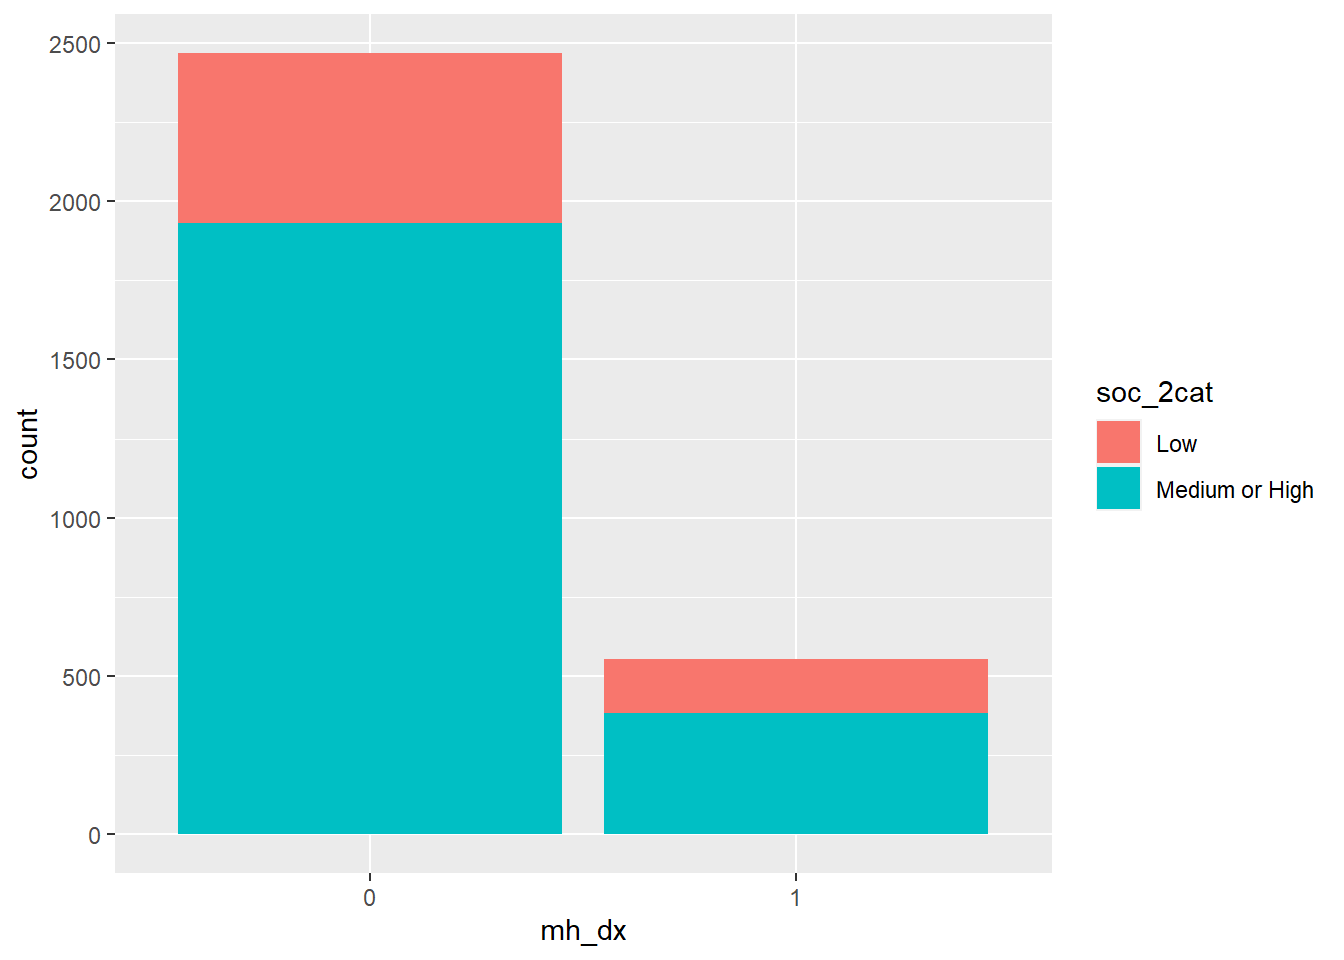
\includegraphics{BMIN503_Final_Project_Craig_files/figure-latex/unnamed-chunk-4-1.pdf}

\begin{Shaded}
\begin{Highlighting}[]
\KeywordTok{describe.by}\NormalTok{(hisp)}
\end{Highlighting}
\end{Shaded}

\begin{verbatim}
##                              vars   n   mean     sd median trimmed    mad
## Race.Ethnicity*                 1 264   1.00   0.00      1    1.00   0.00
## Arrive.to.1st.Med.Given         2 232 177.42  93.04    155  164.38  65.23
## ED.LOS..min.*                   3 263 253.08 143.07    225  238.79 134.92
## Arrive.to.Room                  4 264  25.06  34.85     10   17.32  11.12
## Room.to.MD.Eval                 5 264  22.30  30.71      9   16.01  11.86
## MD.Eval.to.First.Med.Order      6 232  55.79  52.53     43   47.18  29.65
## X1st.Med.Ordered.to.Started*    7 232  96.87  27.78     95   96.65  21.50
## X1st.Med.Started.to.Given*      8 232 121.64  81.05    140  122.08  92.66
## X1st.Med.Reassessment           9 173  71.27  50.83     56   62.98  35.58
##                              min max range  skew kurtosis   se
## Race.Ethnicity*                1   1     0   NaN      NaN 0.00
## Arrive.to.1st.Med.Given       39 831   792  2.38    10.73 6.11
## ED.LOS..min.*                 15 631   616  0.78    -0.08 8.82
## Arrive.to.Room                 0 193   193  2.45     6.55 2.14
## Room.to.MD.Eval               -3 196   199  2.61     8.99 1.89
## MD.Eval.to.First.Med.Order   -80 332   412  2.19     6.99 3.45
## X1st.Med.Ordered.to.Started*   4 157   153 -0.08     0.54 1.82
## X1st.Med.Started.to.Given*     1 258   257 -0.23    -1.28 5.32
## X1st.Med.Reassessment         20 317   297  2.19     6.36 3.86
\end{verbatim}

\begin{Shaded}
\begin{Highlighting}[]
\KeywordTok{hist}\NormalTok{(hisp}\OperatorTok{$}\NormalTok{Arrive.to.1st.Med.Given)}
\end{Highlighting}
\end{Shaded}

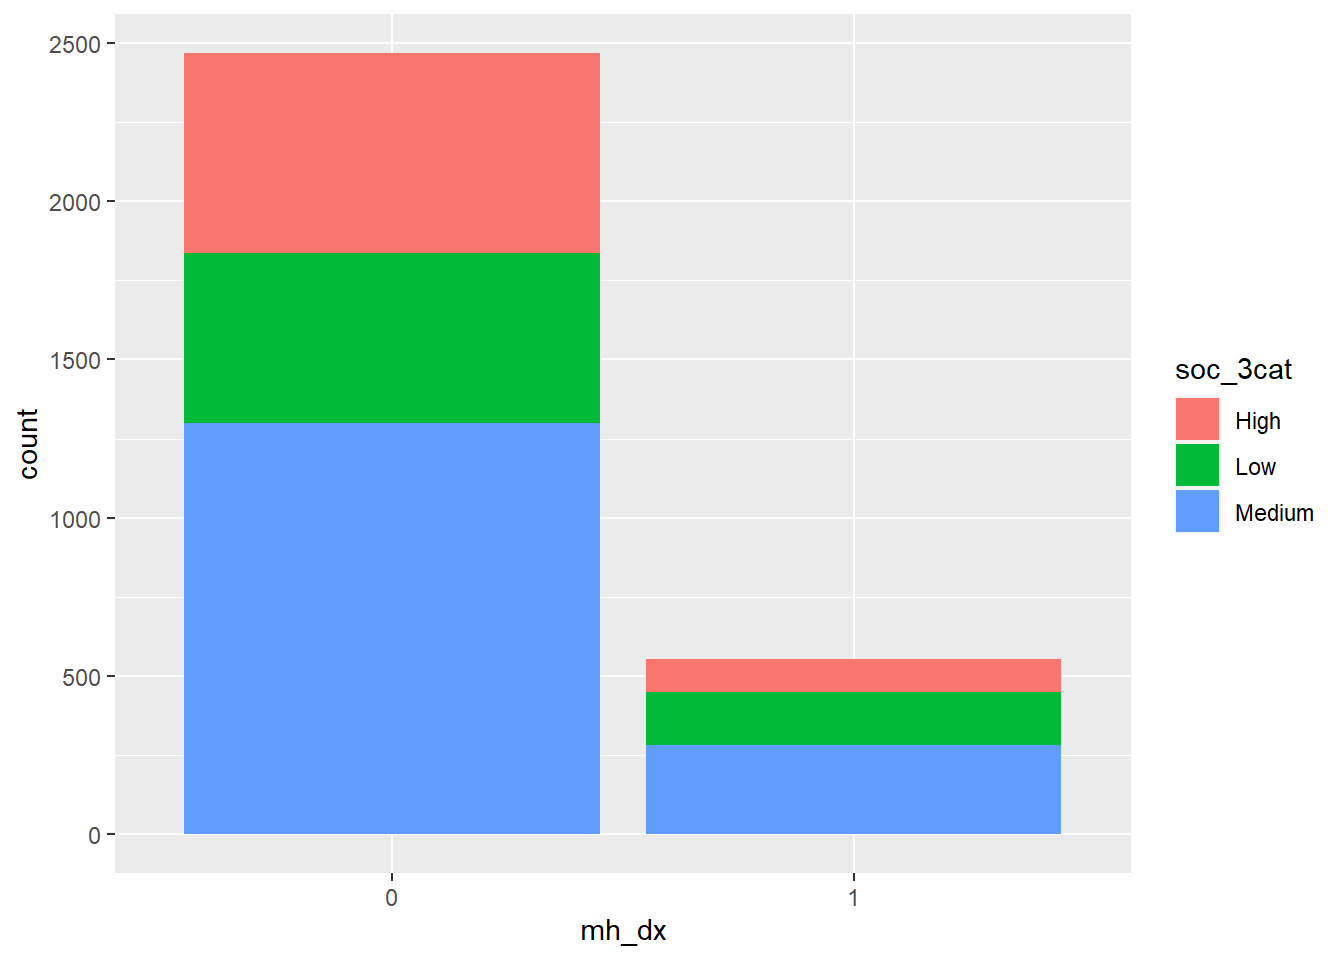
\includegraphics{BMIN503_Final_Project_Craig_files/figure-latex/unnamed-chunk-4-2.pdf}

\begin{Shaded}
\begin{Highlighting}[]
\KeywordTok{describe.by}\NormalTok{(nhw)}
\end{Highlighting}
\end{Shaded}

\begin{verbatim}
##                              vars    n   mean     sd median trimmed    mad
## Race.Ethnicity*                 1 1750   3.00   0.00      3    3.00   0.00
## Arrive.to.1st.Med.Given         2 1578 164.16  87.37    143  152.28  66.72
## ED.LOS..min.*                   3 1750 253.61 133.29    228  243.14 131.21
## Arrive.to.Room                  4 1750  23.87  36.23      9   15.42   8.90
## Room.to.MD.Eval                 5 1750  18.04  26.07      8   12.41  10.38
## MD.Eval.to.First.Med.Order      6 1578  47.34  49.45     37   40.37  26.69
## X1st.Med.Ordered.to.Started*    7 1578  93.43  24.37     92   93.25  17.79
## X1st.Med.Started.to.Given*      8 1578 127.58  79.10    145  129.50  86.73
## X1st.Med.Reassessment           9 1231  70.48  48.79     57   62.11  31.13
##                              min max range  skew kurtosis   se
## Race.Ethnicity*                3   3     0   NaN      NaN 0.00
## Arrive.to.1st.Med.Given       18 835   817  1.83     6.16 2.20
## ED.LOS..min.*                  1 630   629  0.62    -0.30 3.19
## Arrive.to.Room               -56 362   418  2.88    11.16 0.87
## Room.to.MD.Eval              -15 258   273  3.04    13.43 0.62
## MD.Eval.to.First.Med.Order   -96 536   632  2.55    13.33 1.24
## X1st.Med.Ordered.to.Started*   2 163   161  0.00     0.93 0.61
## X1st.Med.Started.to.Given*     1 258   257 -0.33    -1.15 1.99
## X1st.Med.Reassessment         20 521   501  2.59    11.04 1.39
\end{verbatim}

\begin{Shaded}
\begin{Highlighting}[]
\KeywordTok{hist}\NormalTok{(nhw}\OperatorTok{$}\NormalTok{Arrive.to.1st.Med.Given)}
\end{Highlighting}
\end{Shaded}

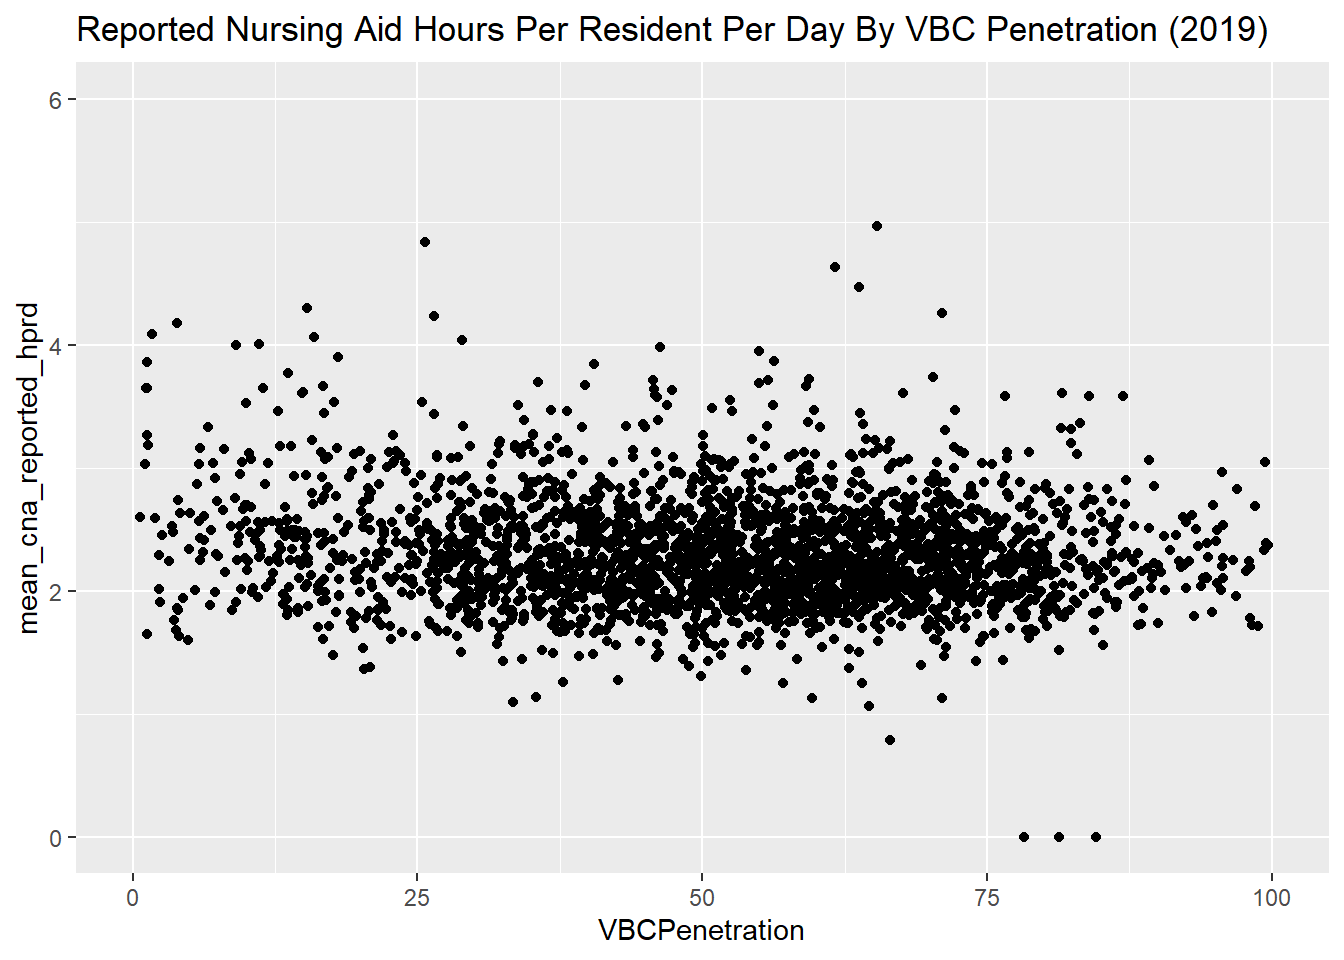
\includegraphics{BMIN503_Final_Project_Craig_files/figure-latex/unnamed-chunk-4-3.pdf}

\begin{Shaded}
\begin{Highlighting}[]
\KeywordTok{describe.by}\NormalTok{(nhb)}
\end{Highlighting}
\end{Shaded}

\begin{verbatim}
##                              vars    n   mean     sd median trimmed    mad
## Race.Ethnicity*                 1 1514   2.00   0.00      2    2.00   0.00
## Arrive.to.1st.Med.Given         2 1296 159.88  81.76    143  149.96  66.72
## ED.LOS..min.*                   3 1514 218.89 138.87    185  202.97 117.87
## Arrive.to.Room                  4 1514  25.64  38.61     10   16.79  11.86
## Room.to.MD.Eval                 5 1514  20.36  28.01     10   14.66  11.86
## MD.Eval.to.First.Med.Order      6 1296  48.80  46.77     37   41.24  26.69
## X1st.Med.Ordered.to.Started*    7 1296  92.32  25.63     91   91.63  19.27
## X1st.Med.Started.to.Given*      8 1296 113.95  84.44    123  112.42 115.64
## X1st.Med.Reassessment           9  915  65.77  44.10     55   59.05  28.17
##                               min max range  skew kurtosis   se
## Race.Ethnicity*                 2   2     0   NaN      NaN 0.00
## Arrive.to.1st.Med.Given        26 640   614  1.62     4.37 2.27
## ED.LOS..min.*                   2 637   635  1.01     0.57 3.57
## Arrive.to.Room                -51 405   456  3.18    14.49 0.99
## Room.to.MD.Eval               -13 293   306  3.12    15.59 0.72
## MD.Eval.to.First.Med.Order   -128 361   489  2.28     8.80 1.30
## X1st.Med.Ordered.to.Started*    3 163   160  0.16     0.53 0.71
## X1st.Med.Started.to.Given*      1 258   257 -0.09    -1.39 2.35
## X1st.Med.Reassessment          20 486   466  3.25    18.44 1.46
\end{verbatim}

\begin{Shaded}
\begin{Highlighting}[]
\KeywordTok{hist}\NormalTok{(nhb}\OperatorTok{$}\NormalTok{Arrive.to.1st.Med.Given)}
\end{Highlighting}
\end{Shaded}

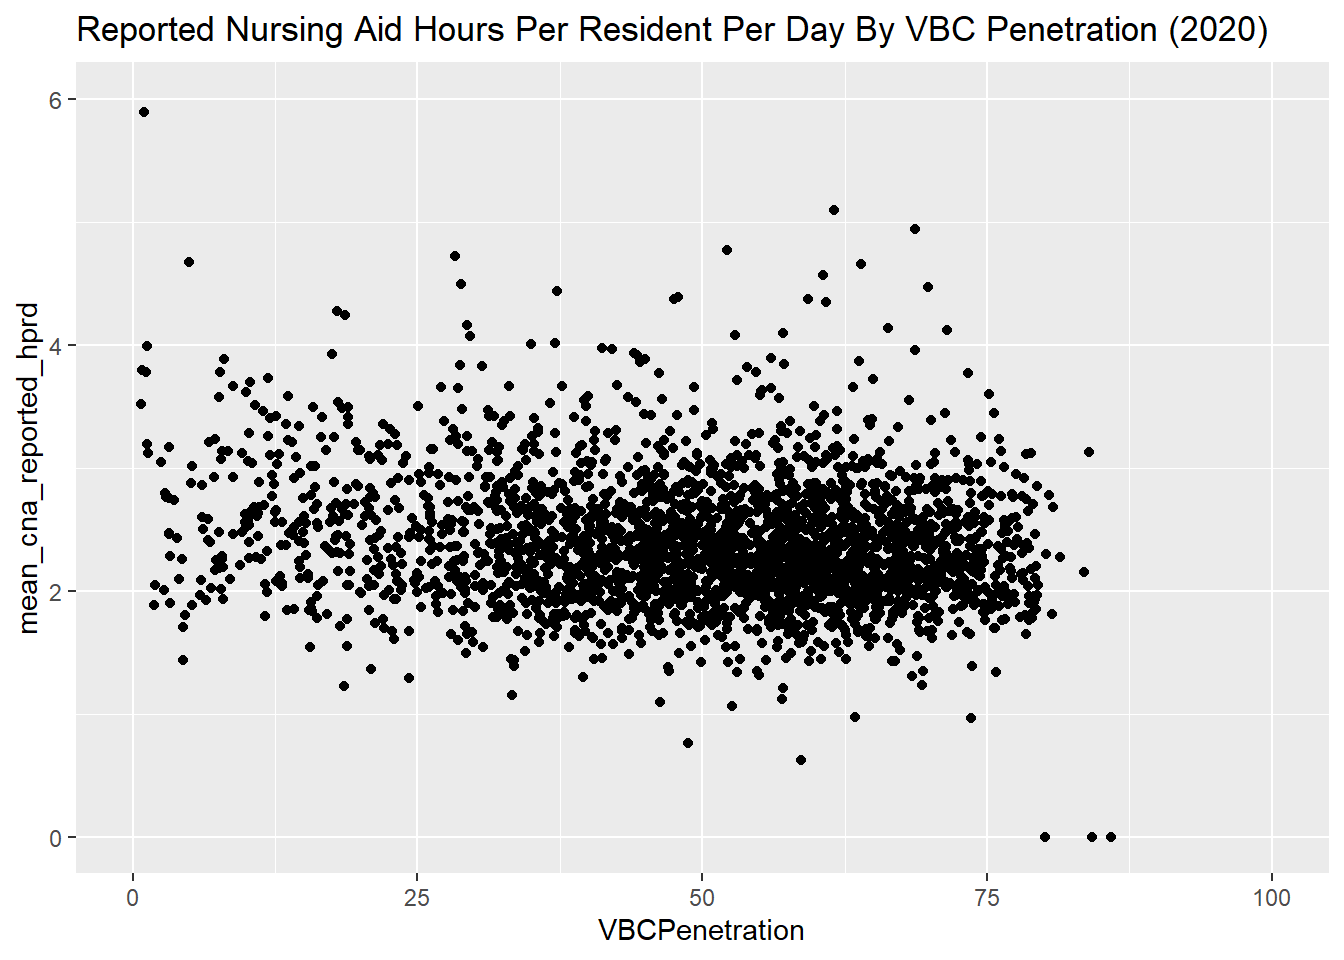
\includegraphics{BMIN503_Final_Project_Craig_files/figure-latex/unnamed-chunk-4-4.pdf}

\begin{Shaded}
\begin{Highlighting}[]
\KeywordTok{describe.by}\NormalTok{(other)}
\end{Highlighting}
\end{Shaded}

\begin{verbatim}
##                              vars   n   mean     sd median trimmed    mad
## Race.Ethnicity*                 1 181   4.00   0.00    4.0    4.00   0.00
## Arrive.to.1st.Med.Given         2 152 160.39  82.81  143.0  149.48  58.56
## ED.LOS..min.*                   3 181 237.08 139.92  207.0  223.82 133.43
## Arrive.to.Room                  4 181  27.17  35.26   10.0   20.03  10.38
## Room.to.MD.Eval                 5 181  20.60  24.91   12.0   15.54  16.31
## MD.Eval.to.First.Med.Order      6 152  47.18  59.26   32.5   37.07  20.02
## X1st.Med.Ordered.to.Started*    7 152  91.67  25.72   91.0   92.10  17.79
## X1st.Med.Started.to.Given*      8 152 117.84  84.71  131.0  117.25 105.26
## X1st.Med.Reassessment           9 112  70.76  47.11   62.0   62.22  28.91
##                              min max range  skew kurtosis    se
## Race.Ethnicity*                4   4     0   NaN      NaN  0.00
## Arrive.to.1st.Med.Given       46 593   547  1.77     4.96  6.72
## ED.LOS..min.*                 28 615   587  0.75    -0.27 10.40
## Arrive.to.Room                 0 207   207  1.99     4.43  2.62
## Room.to.MD.Eval               -2 123   125  1.91     3.80  1.85
## MD.Eval.to.First.Med.Order   -69 498   567  4.20    24.82  4.81
## X1st.Med.Ordered.to.Started*   1 153   152 -0.34     1.17  2.09
## X1st.Med.Started.to.Given*     1 253   252 -0.15    -1.43  6.87
## X1st.Med.Reassessment         20 300   280  2.12     5.59  4.45
\end{verbatim}

\begin{Shaded}
\begin{Highlighting}[]
\KeywordTok{hist}\NormalTok{(other}\OperatorTok{$}\NormalTok{Arrive.to.1st.Med.Given)}
\end{Highlighting}
\end{Shaded}

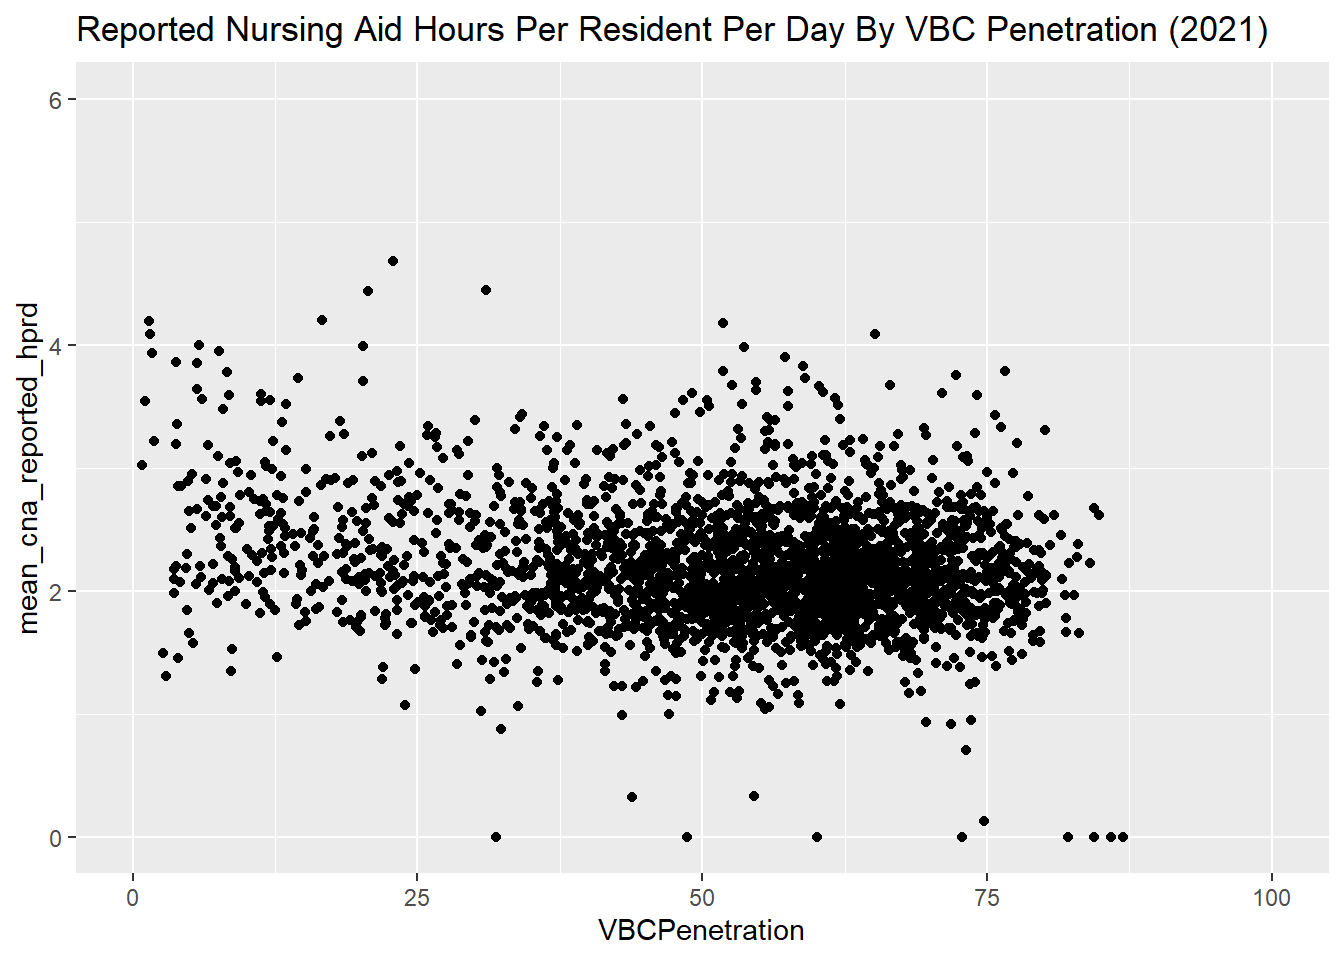
\includegraphics{BMIN503_Final_Project_Craig_files/figure-latex/unnamed-chunk-4-5.pdf}

Contingency (two-way) tables: Group table one variables by race and eth

\begin{Shaded}
\begin{Highlighting}[]
\NormalTok{race_eth_all <-}\StringTok{ }\NormalTok{data_all_na}\OperatorTok{$}\NormalTok{Race.Ethnicity}
\NormalTok{payer_type <-}\StringTok{ }\NormalTok{data_all_na}\OperatorTok{$}\NormalTok{Payer.Type}
\NormalTok{sex_all <-}\StringTok{ }\NormalTok{data_all_na}\OperatorTok{$}\NormalTok{Sex}
\NormalTok{pth_all <-}\StringTok{ }\NormalTok{data_all_na}\OperatorTok{$}\NormalTok{Pathway}
\NormalTok{lng_all <-}\StringTok{ }\NormalTok{data_all_na}\OperatorTok{$}\NormalTok{Primary.Language}
\NormalTok{acu_all <-}\StringTok{ }\NormalTok{data_all_na}\OperatorTok{$}\NormalTok{Acuity}
\NormalTok{dis_all <-}\StringTok{ }\NormalTok{data_all_na}\OperatorTok{$}\NormalTok{Dispo}
\NormalTok{team_all <-}\StringTok{ }\NormalTok{data_all_na}\OperatorTok{$}\NormalTok{Team.Assessment.}
\NormalTok{arr_all <-}\StringTok{ }\NormalTok{data_all_na}\OperatorTok{$}\NormalTok{Arrive.to.1st.Med.Given}

\NormalTok{payer_by_tab <-}\StringTok{ }\KeywordTok{addmargins}\NormalTok{(}\KeywordTok{table}\NormalTok{(race_eth_all, payer_type)) }\CommentTok{#n's for each group}
\KeywordTok{print}\NormalTok{(payer_by_tab)}
\end{Highlighting}
\end{Shaded}

\begin{verbatim}
##                     payer_type
## race_eth_all         COMMERCIAL MEDICAL ASSISTANCE  Sum
##   HISPANIC OR LATINO        114                134  248
##   NON-HISPANIC BLACK        445               1020 1465
##   NON-HISPANIC WHITE       1422                287 1709
##   OTHER                     108                 67  175
##   Sum                      2089               1508 3597
\end{verbatim}

\begin{Shaded}
\begin{Highlighting}[]
\KeywordTok{prop.table}\NormalTok{(payer_by_tab,}\DecValTok{2}\NormalTok{)}\OperatorTok
\StringTok{  }\KeywordTok{round}\NormalTok{ (}\DataTypeTok{digits =}\DecValTok{2}\NormalTok{) }\CommentTok{# column pcts ie race/eth}
\end{Highlighting}
\end{Shaded}

\begin{verbatim}
##                     payer_type
## race_eth_all         COMMERCIAL MEDICAL ASSISTANCE  Sum
##   HISPANIC OR LATINO       0.03               0.04 0.03
##   NON-HISPANIC BLACK       0.11               0.34 0.20
##   NON-HISPANIC WHITE       0.34               0.10 0.24
##   OTHER                    0.03               0.02 0.02
##   Sum                      0.50               0.50 0.50
\end{verbatim}

\begin{Shaded}
\begin{Highlighting}[]
\KeywordTok{prop.table}\NormalTok{(payer_by_tab,}\DecValTok{1}\NormalTok{)}\OperatorTok
\StringTok{  }\KeywordTok{round}\NormalTok{ (}\DataTypeTok{digits =}\DecValTok{2}\NormalTok{) }\CommentTok{# row pcts ie payer type. which one is the best way to display this data ***}
\end{Highlighting}
\end{Shaded}

\begin{verbatim}
##                     payer_type
## race_eth_all         COMMERCIAL MEDICAL ASSISTANCE  Sum
##   HISPANIC OR LATINO       0.23               0.27 0.50
##   NON-HISPANIC BLACK       0.15               0.35 0.50
##   NON-HISPANIC WHITE       0.42               0.08 0.50
##   OTHER                    0.31               0.19 0.50
##   Sum                      0.29               0.21 0.50
\end{verbatim}

\begin{Shaded}
\begin{Highlighting}[]
\NormalTok{sex_by_tab <-}\StringTok{ }\KeywordTok{table}\NormalTok{(race_eth_all, sex_all) }
\KeywordTok{prop.table}\NormalTok{(sex_by_tab,}\DecValTok{2}\NormalTok{)}\OperatorTok
\StringTok{  }\KeywordTok{round}\NormalTok{ (}\DataTypeTok{digits =}\DecValTok{2}\NormalTok{) }\CommentTok{#more black males than white males have migraines?? ***}
\end{Highlighting}
\end{Shaded}

\begin{verbatim}
##                     sex_all
## race_eth_all            F    M
##   HISPANIC OR LATINO 0.07 0.07
##   NON-HISPANIC BLACK 0.39 0.45
##   NON-HISPANIC WHITE 0.49 0.42
##   OTHER              0.04 0.06
\end{verbatim}

\begin{Shaded}
\begin{Highlighting}[]
\KeywordTok{prop.table}\NormalTok{(sex_by_tab,}\DecValTok{1}\NormalTok{)}\OperatorTok
\StringTok{  }\KeywordTok{round}\NormalTok{ (}\DataTypeTok{digits =}\DecValTok{2}\NormalTok{) }\CommentTok{#makes more sense}
\end{Highlighting}
\end{Shaded}

\begin{verbatim}
##                     sex_all
## race_eth_all            F    M
##   HISPANIC OR LATINO 0.72 0.28
##   NON-HISPANIC BLACK 0.67 0.33
##   NON-HISPANIC WHITE 0.74 0.26
##   OTHER              0.64 0.36
\end{verbatim}

\begin{Shaded}
\begin{Highlighting}[]
\NormalTok{pth_by_tab <-}\StringTok{ }\KeywordTok{table}\NormalTok{(race_eth_all,pth_all) }
\KeywordTok{prop.table}\NormalTok{(pth_by_tab,}\DecValTok{2}\NormalTok{) }\OperatorTok
\StringTok{  }\KeywordTok{round}\NormalTok{ (}\DataTypeTok{digits =}\DecValTok{2}\NormalTok{)}
\end{Highlighting}
\end{Shaded}

\begin{verbatim}
##                     pth_all
## race_eth_all           No  Yes
##   HISPANIC OR LATINO 0.07 0.07
##   NON-HISPANIC BLACK 0.48 0.39
##   NON-HISPANIC WHITE 0.40 0.49
##   OTHER              0.05 0.05
\end{verbatim}

\begin{Shaded}
\begin{Highlighting}[]
\KeywordTok{prop.table}\NormalTok{(pth_by_tab,}\DecValTok{1}\NormalTok{)  }\OperatorTok
\StringTok{  }\KeywordTok{round}\NormalTok{ (}\DataTypeTok{digits =}\DecValTok{2}\NormalTok{)}
\end{Highlighting}
\end{Shaded}

\begin{verbatim}
##                     pth_all
## race_eth_all           No  Yes
##   HISPANIC OR LATINO 0.17 0.83
##   NON-HISPANIC BLACK 0.21 0.79
##   NON-HISPANIC WHITE 0.15 0.85
##   OTHER              0.17 0.83
\end{verbatim}

\begin{Shaded}
\begin{Highlighting}[]
\NormalTok{lng_by_tab <-}\StringTok{ }\KeywordTok{table}\NormalTok{(race_eth_all, lng_all)}
\KeywordTok{prop.table}\NormalTok{(lng_by_tab,}\DecValTok{2}\NormalTok{)}\OperatorTok
\StringTok{  }\KeywordTok{round}\NormalTok{ (}\DataTypeTok{digits =}\DecValTok{2}\NormalTok{)}
\end{Highlighting}
\end{Shaded}

\begin{verbatim}
##                     lng_all
## race_eth_all         ENGLISH NON-ENGLISH
##   HISPANIC OR LATINO    0.06        0.54
##   NON-HISPANIC BLACK    0.41        0.04
##   NON-HISPANIC WHITE    0.48        0.09
##   OTHER                 0.04        0.32
\end{verbatim}

\begin{Shaded}
\begin{Highlighting}[]
\KeywordTok{prop.table}\NormalTok{(lng_by_tab,}\DecValTok{1}\NormalTok{)}\OperatorTok
\StringTok{  }\KeywordTok{round}\NormalTok{ (}\DataTypeTok{digits =}\DecValTok{2}\NormalTok{)}
\end{Highlighting}
\end{Shaded}

\begin{verbatim}
##                     lng_all
## race_eth_all         ENGLISH NON-ENGLISH
##   HISPANIC OR LATINO    0.86        0.14
##   NON-HISPANIC BLACK    1.00        0.00
##   NON-HISPANIC WHITE    1.00        0.00
##   OTHER                 0.88        0.12
\end{verbatim}

\begin{Shaded}
\begin{Highlighting}[]
\NormalTok{acu_by_tab <-}\StringTok{ }\KeywordTok{addmargins}\NormalTok{(}\KeywordTok{table}\NormalTok{(race_eth_all, acu_all))}
\KeywordTok{print}\NormalTok{(acu_by_tab)}
\end{Highlighting}
\end{Shaded}

\begin{verbatim}
##                     acu_all
## race_eth_all         1 Critical 2 Acute 3 Urgent 4 Urgent 5 Non-Urgent
##   HISPANIC OR LATINO          0      58      180       24            2
##   NON-HISPANIC BLACK          1     207     1060      237            9
##   NON-HISPANIC WHITE          5     334     1376       35            0
##   OTHER                       1      24      137       16            3
##   Sum                         7     623     2753      312           14
##                     acu_all
## race_eth_all          Sum
##   HISPANIC OR LATINO  264
##   NON-HISPANIC BLACK 1514
##   NON-HISPANIC WHITE 1750
##   OTHER               181
##   Sum                3709
\end{verbatim}

\begin{Shaded}
\begin{Highlighting}[]
\NormalTok{acu_by_tab_p <-}\KeywordTok{table}\NormalTok{(race_eth_all, acu_all)}
\KeywordTok{prop.table}\NormalTok{(acu_by_tab_p,}\DecValTok{2}\NormalTok{) }\OperatorTok
\StringTok{  }\KeywordTok{round}\NormalTok{ (}\DataTypeTok{digits =}\DecValTok{2}\NormalTok{)}
\end{Highlighting}
\end{Shaded}

\begin{verbatim}
##                     acu_all
## race_eth_all         1 Critical 2 Acute 3 Urgent 4 Urgent 5 Non-Urgent
##   HISPANIC OR LATINO       0.00    0.09     0.07     0.08         0.14
##   NON-HISPANIC BLACK       0.14    0.33     0.39     0.76         0.64
##   NON-HISPANIC WHITE       0.71    0.54     0.50     0.11         0.00
##   OTHER                    0.14    0.04     0.05     0.05         0.21
\end{verbatim}

\begin{Shaded}
\begin{Highlighting}[]
\KeywordTok{prop.table}\NormalTok{(acu_by_tab_p,}\DecValTok{1}\NormalTok{)}\OperatorTok
\StringTok{  }\KeywordTok{round}\NormalTok{ (}\DataTypeTok{digits =}\DecValTok{2}\NormalTok{)}
\end{Highlighting}
\end{Shaded}

\begin{verbatim}
##                     acu_all
## race_eth_all         1 Critical 2 Acute 3 Urgent 4 Urgent 5 Non-Urgent
##   HISPANIC OR LATINO       0.00    0.22     0.68     0.09         0.01
##   NON-HISPANIC BLACK       0.00    0.14     0.70     0.16         0.01
##   NON-HISPANIC WHITE       0.00    0.19     0.79     0.02         0.00
##   OTHER                    0.01    0.13     0.76     0.09         0.02
\end{verbatim}

\begin{Shaded}
\begin{Highlighting}[]
\NormalTok{dis_by_tab <-}\StringTok{ }\KeywordTok{addmargins}\NormalTok{(}\KeywordTok{table}\NormalTok{(race_eth_all, dis_all))}
\KeywordTok{print}\NormalTok{(dis_by_tab)}
\end{Highlighting}
\end{Shaded}

\begin{verbatim}
##                     dis_all
## race_eth_all         Admitted Discharged  Sum
##   HISPANIC OR LATINO       40        224  264
##   NON-HISPANIC BLACK      157       1357 1514
##   NON-HISPANIC WHITE      372       1378 1750
##   OTHER                    28        153  181
##   Sum                     597       3112 3709
\end{verbatim}

\begin{Shaded}
\begin{Highlighting}[]
\NormalTok{dis_by_tab_p <-}\KeywordTok{table}\NormalTok{(race_eth_all, dis_all)}
\KeywordTok{prop.table}\NormalTok{(dis_by_tab_p,}\DecValTok{2}\NormalTok{) }\OperatorTok
\StringTok{  }\KeywordTok{round}\NormalTok{ (}\DataTypeTok{digits =}\DecValTok{2}\NormalTok{)}
\end{Highlighting}
\end{Shaded}

\begin{verbatim}
##                     dis_all
## race_eth_all         Admitted Discharged
##   HISPANIC OR LATINO     0.07       0.07
##   NON-HISPANIC BLACK     0.26       0.44
##   NON-HISPANIC WHITE     0.62       0.44
##   OTHER                  0.05       0.05
\end{verbatim}

\begin{Shaded}
\begin{Highlighting}[]
\KeywordTok{prop.table}\NormalTok{(dis_by_tab_p,}\DecValTok{1}\NormalTok{)}\OperatorTok
\StringTok{  }\KeywordTok{round}\NormalTok{ (}\DataTypeTok{digits =}\DecValTok{2}\NormalTok{)}
\end{Highlighting}
\end{Shaded}

\begin{verbatim}
##                     dis_all
## race_eth_all         Admitted Discharged
##   HISPANIC OR LATINO     0.15       0.85
##   NON-HISPANIC BLACK     0.10       0.90
##   NON-HISPANIC WHITE     0.21       0.79
##   OTHER                  0.15       0.85
\end{verbatim}

\begin{Shaded}
\begin{Highlighting}[]
\CommentTok{#Arrival to first med given in minutes, grouped by race/eth}
\NormalTok{arr_group_by_all <-}\StringTok{ }\NormalTok{data_all_na }\OperatorTok
\StringTok{  }\KeywordTok{group_by}\NormalTok{(Race.Ethnicity) }\OperatorTok
\StringTok{  }\KeywordTok{summarise}\NormalTok{(}\DataTypeTok{mean_arr =} \KeywordTok{mean}\NormalTok{(Arrive.to.1st.Med.Given, }\DataTypeTok{na.rm =} \OtherTok{TRUE}\NormalTok{),}
            \DataTypeTok{sd_arr =} \KeywordTok{sd}\NormalTok{(Arrive.to.1st.Med.Given, }\DataTypeTok{na.rm =} \OtherTok{TRUE}\NormalTok{),}
            \DataTypeTok{med_arr =} \KeywordTok{median}\NormalTok{(Arrive.to.1st.Med.Given, }\DataTypeTok{na.rm =} \OtherTok{TRUE}\NormalTok{ ),}
            \DataTypeTok{min_arr =} \KeywordTok{min}\NormalTok{(Arrive.to.1st.Med.Given, }\DataTypeTok{na.rm =} \OtherTok{TRUE}\NormalTok{ ),}
            \DataTypeTok{max_arr =} \KeywordTok{max}\NormalTok{(Arrive.to.1st.Med.Given, }\DataTypeTok{na.rm =} \OtherTok{TRUE}\NormalTok{ )) }\OperatorTok
\StringTok{  }\NormalTok{return}

\KeywordTok{print.data.frame}\NormalTok{(arr_group_by_all)}
\end{Highlighting}
\end{Shaded}

\begin{verbatim}
##       Race.Ethnicity mean_arr   sd_arr med_arr min_arr max_arr
## 1 HISPANIC OR LATINO 177.4224 93.03745     155      39     831
## 2 NON-HISPANIC BLACK 159.8750 81.76349     143      26     640
## 3 NON-HISPANIC WHITE 164.1565 87.37185     143      18     835
## 4              OTHER 160.3882 82.81489     143      46     593
\end{verbatim}

\subsubsection{Statistical Analyses}\label{statistical-analyses}

\paragraph{Linear regression models: data set of select variables
without
NAs}\label{linear-regression-models-data-set-of-select-variables-without-nas}

\begin{Shaded}
\begin{Highlighting}[]
\CommentTok{#Make a data set of select variables without NAs}
\NormalTok{data_select_clean <-}\StringTok{ }\NormalTok{data_select[}\KeywordTok{complete.cases}\NormalTok{(data_select[ , ]),]}\OperatorTok
\StringTok{  }\KeywordTok{mutate}\NormalTok{(}\DataTypeTok{Team.Assessment.=}\KeywordTok{factor}\NormalTok{(Team.Assessment., }\DataTypeTok{levels=}\KeywordTok{c}\NormalTok{(}\DecValTok{0}\NormalTok{, }\DecValTok{1}\NormalTok{), }\DataTypeTok{labels=}\KeywordTok{c}\NormalTok{(}\StringTok{"no"}\NormalTok{, }\StringTok{"yes"}\NormalTok{))) }\OperatorTok
\StringTok{  }\NormalTok{return}

\KeywordTok{ggplot}\NormalTok{(data_select_clean, }\KeywordTok{aes}\NormalTok{(}\DataTypeTok{x=}\NormalTok{Race.Ethnicity, }\DataTypeTok{y=}\NormalTok{ Arrive.to.1st.Med.Given))}\OperatorTok{+}
\StringTok{  }\KeywordTok{geom_boxplot}\NormalTok{(}\DataTypeTok{color=}\StringTok{"black"}\NormalTok{, }\DataTypeTok{fill=}\StringTok{"lightblue"}\NormalTok{)}
\end{Highlighting}
\end{Shaded}

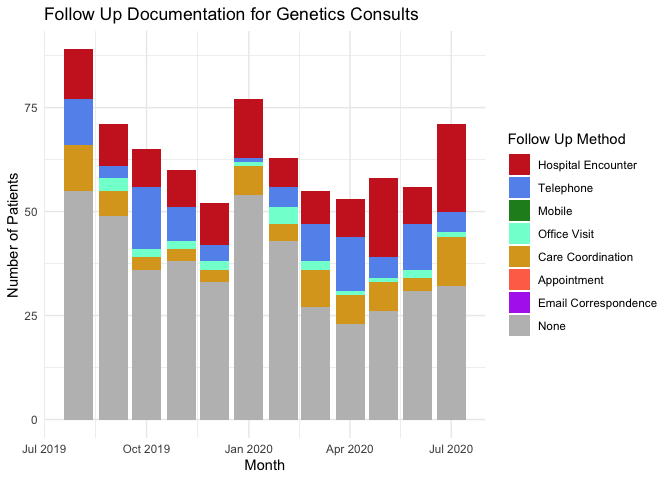
\includegraphics{BMIN503_Final_Project_Craig_files/figure-latex/unnamed-chunk-6-1.pdf}

\begin{Shaded}
\begin{Highlighting}[]
\NormalTok{data_fit <-}\StringTok{ }\KeywordTok{lm}\NormalTok{(Arrive.to.1st.Med.Given }\OperatorTok{~}\StringTok{ }\NormalTok{Race.Ethnicity, }\DataTypeTok{data=}\NormalTok{data_select_clean)}
\KeywordTok{summary}\NormalTok{(data_fit) }\CommentTok{#So the odds when the demographic is "0" or not defined, is 258 minutes? the odds of arrival to first med given for any er pt of a non predetermined race is 258 minutes??? What happened to Hispanic group?}
\end{Highlighting}
\end{Shaded}

\begin{verbatim}
## 
## Call:
## lm(formula = Arrive.to.1st.Med.Given ~ Race.Ethnicity, data = data_select_clean)
## 
## Residuals:
##     Min      1Q  Median      3Q     Max 
## -146.23  -58.33  -19.23   35.72  670.77 
## 
## Coefficients:
##                                  Estimate Std. Error t value Pr(>|t|)    
## (Intercept)                       180.009      5.782  31.133  < 2e-16 ***
## Race.EthnicityNON-HISPANIC BLACK  -19.681      6.264  -3.142  0.00169 ** 
## Race.EthnicityNON-HISPANIC WHITE  -15.777      6.178  -2.554  0.01070 *  
## Race.EthnicityOTHER               -24.145      9.111  -2.650  0.00809 ** 
## ---
## Signif. codes:  0 '***' 0.001 '**' 0.01 '*' 0.05 '.' 0.1 ' ' 1
## 
## Residual standard error: 85.37 on 3155 degrees of freedom
## Multiple R-squared:  0.003527,   Adjusted R-squared:  0.00258 
## F-statistic: 3.722 on 3 and 3155 DF,  p-value: 0.01094
\end{verbatim}

\begin{Shaded}
\begin{Highlighting}[]
\KeywordTok{coef}\NormalTok{(data_fit) }\CommentTok{#Coefficients of X}
\end{Highlighting}
\end{Shaded}

\begin{verbatim}
##                      (Intercept) Race.EthnicityNON-HISPANIC BLACK 
##                        180.00917                        -19.68142 
## Race.EthnicityNON-HISPANIC WHITE              Race.EthnicityOTHER 
##                        -15.77671                        -24.14523
\end{verbatim}

\begin{Shaded}
\begin{Highlighting}[]
\KeywordTok{confint}\NormalTok{(data_fit) }\CommentTok{#Confidence intervals}
\end{Highlighting}
\end{Shaded}

\begin{verbatim}
##                                      2.5 %     97.5 %
## (Intercept)                      168.67228 191.346072
## Race.EthnicityNON-HISPANIC BLACK -31.96428  -7.398567
## Race.EthnicityNON-HISPANIC WHITE -27.88947  -3.663942
## Race.EthnicityOTHER              -42.00936  -6.281094
\end{verbatim}

\begin{Shaded}
\begin{Highlighting}[]
\KeywordTok{summary.lm}\NormalTok{(}\KeywordTok{lm}\NormalTok{(Arrive.to.1st.Med.Given }\OperatorTok{~}\StringTok{ }\NormalTok{Race.Ethnicity }\OperatorTok{+}\StringTok{ }\NormalTok{Acuity, }\DataTypeTok{data=}\NormalTok{data_select_clean))}
\end{Highlighting}
\end{Shaded}

\begin{verbatim}
## 
## Call:
## lm(formula = Arrive.to.1st.Med.Given ~ Race.Ethnicity + Acuity, 
##     data = data_select_clean)
## 
## Residuals:
##     Min      1Q  Median      3Q     Max 
## -174.67  -58.00  -19.73   36.93  674.27 
## 
## Coefficients:
##                                  Estimate Std. Error t value Pr(>|t|)    
## (Intercept)                       260.860     42.941   6.075 1.39e-09 ***
## Race.EthnicityNON-HISPANIC BLACK  -17.856      6.259  -2.853  0.00436 ** 
## Race.EthnicityNON-HISPANIC WHITE  -15.194      6.166  -2.464  0.01378 *  
## Race.EthnicityOTHER               -21.995      9.096  -2.418  0.01566 *  
## Acuity2 Acute                     -65.919     42.683  -1.544  0.12260    
## Acuity3 Urgent                    -84.933     42.559  -1.996  0.04606 *  
## Acuity4 Urgent                    -89.604     43.011  -2.083  0.03731 *  
## Acuity5 Non-Urgent               -135.748     57.142  -2.376  0.01758 *  
## ---
## Signif. codes:  0 '***' 0.001 '**' 0.01 '*' 0.05 '.' 0.1 ' ' 1
## 
## Residual standard error: 85.03 on 3151 degrees of freedom
## Multiple R-squared:  0.01264,    Adjusted R-squared:  0.01044 
## F-statistic: 5.762 on 7 and 3151 DF,  p-value: 1.201e-06
\end{verbatim}


\end{document}
